
% ==============================================================================
% ==============================================================================
%
% HEADER
%
% ==============================================================================
% ==============================================================================

\documentclass{article}

\usepackage[T1]{fontenc}
\usepackage[utf8]{inputenc}
\usepackage[english]{babel}
\usepackage{graphicx}

\usepackage[
backend=biber,
%style=alphabetic,
%citestyle=authoryear
]{biblatex}

\usepackage{amssymb}
\usepackage{amsmath}
\usepackage{bm} % bold maths symbols
\usepackage{graphicx}
\usepackage{float}
\usepackage{hyperref}
\usepackage{algorithm}
\usepackage{algpseudocode}


\usepackage[a4paper, total={7in, 10in}]{geometry}


% ==============================================================================
% ==============================================================================
%
% DEFINITIONS
%
% ==============================================================================
% ==============================================================================
\addbibresource{cite.bib}


\renewcommand{\vec}[1]{\mathbf{#1}}
\renewcommand{\d}{\,\text{d}}


\newcommand{\A}{\mathcal{A}}
\newcommand{\E}{\mathcal{E}}
\newcommand{\F}{\mathcal{F}}
\renewcommand{\L}{\mathcal{L}}
\newcommand{\X}{\mathcal{X}}

\newcommand{\Enc}{\mathtt{Enc}}
\newcommand{\Dec}{\mathtt{Dec}}

\newcommand{\Oh}{\mathcal{O}}
\newcommand{\KL}[2]{\mathrm{KL}[\,#1\,\,||\,\,#2\,]}
\newcommand{\Exp}{\mathbb{E}}
\newcommand{\I}{\mathbb{I}}

\newcommand{\Hypos}{\mathcal{H}}
\newcommand{\Data}{\mathcal{D}}

\newcommand{\ImSpace}{\mathcal{X}}

\newcommand{\Reals}{\mathbb{R}}
\newcommand{\Ints}{\mathbb{Z}}
\newcommand{\Nats}{\mathbb{N}}

\newcommand{\Norm}[1]{\mathcal{N}\left( #1 \right)}
\newcommand{\Unif}[1]{\mathcal{U}\left( #1 \right)}
\newcommand{\Laplace}[1]{\mathcal{L}\left( #1 \right)}

% Bold maths symbols
\newcommand{\MU}{\boldsymbol\mu}
\newcommand{\SIGMA}{\boldsymbol\sigma}
\newcommand{\PSI}{\boldsymbol\psi}
\newcommand{\THETA}{\boldsymbol\theta}
\newcommand{\PHI}{\boldsymbol\phi}

\DeclareMathOperator*{\argmax}{arg\,max}
\DeclareMathOperator*{\argmin}{arg\,min}


\title{Compression without Quantization}
\author{Gergely Flamich}

% ==============================================================================
% ==============================================================================
%
% START OF THESIS
%
% ==============================================================================
% ==============================================================================

\begin{document}

\input{titlepage.tex}

% ==============================================================================
%
% DECLARATION
%
% ==============================================================================

\vspace{2cm}

\begin{center}
\Huge
\textbf{Declaration}
\end{center}

\vspace{1cm}

\large
\noindent I, Gergely Flamich of St John's College, being a candidate for the
MPhil in Machine Learning and Machine Intelligence, hereby declare that this
report and the work described in it are my own work, unaided except as may be
specified below, and that the report does not contain material that has
already been used to any substantial extent for a comparable purpose.


\vspace{2cm}

\large
\noindent
Wordcount: \textbf{16384} words

\newpage

% ==============================================================================
%
% ACKNOWLEDGEMENTS
%
% ==============================================================================

\vspace{2cm}

\begin{center}
\Huge
\textbf{Acknowledgements}
\end{center}

\vspace{1cm}



\newpage

% ==============================================================================
%
% ABSTRACT
%
% ==============================================================================

\begin{abstract}
  We provide an implementation of our proposed method written in \texttt{Tensorflow}
  \cite{tensorflow2015-whitepaper} and \texttt{Sonnet} \cite{sonnetblog},
  available on GitHub \footnotemark.
\end{abstract}

\footnotetext{https://github.com/gergely-flamich/miracle-compression}

\newpage

\tableofcontents

\newpage

% ==============================================================================
% ==============================================================================
%
% START OF CONTENTS
%
% ==============================================================================
% ==============================================================================

% ==============================================================================
% ==============================================================================
%
% Related work
%
% ==============================================================================
% ==============================================================================

\section{Related Work}
\par
Here we give a brief overview of the history of using machine learning for image
compression. Then, we focus on recent advances in lossy image compression and
describe and compare their methods to each other as well as ours.
\subsection{Machine Learning-based Image Compression}
\par

First attempt by \cite{bottou1998high} DjVu focused on segmenting foreground and
background in magazines and using K-means clustering to analize and code the
background.

Neural network based image compression has been theorized about for a long time
now \cite{mougeot1991image} \cite{jiang1999image} 
\cite{toderici2015variable} focused only 32x32 thumbnails
Image reconstruction through compressive representations \cite{denton2015deep},
\cite{gregor2015draw}

\subsection{Comparison of Recent Works}
\label{sec:lit_comparison}
\par

There have been several recent advances in neural network-based compression
techniques, most notably \cite{toderici2015variable}, \cite{balle2016end},
\cite{toderici2017full}, \cite{theis2017lossy}, \cite{rippel2017real},
\cite{balle2018variational}, \cite{johnston2018cvpr}, \cite{mentzer2018cvpr}. 
An interesting commonality between these approaches is that there is very little
commonality between them, for a multidue of reasons, on which we hope to shed
some lite in this section. Instead of analyzing them in a historical order, we
will instead go through the compression pipeline and compare them head-to-head
in each compartment separately. 
\subsubsection{Datasets and Input Pipelines}
\par
Somewhat surprisingly it appears that there is no canonical dataset (yet) for
the task at hand, namely a set of high-resolution, variable-sized losslessly
encoded colour images,
although CLIC \cite{clic2018} seems to be an emerging one. Perhaps the reason is
that generally in other domains, such as image-based classification cropping and
rescaling images can effectively side-step the need to deal with variable-sized
images. However, when it comes to compression, if we hope to build anything
useful, we must account for this.
\par
On the other hand most authors have used the Kodak dataset \cite{kodakdataset}
for testing / reporting results.
\begin{itemize}
\item \cite{balle2016end} trained on 6507 images, selected from ImageNet
  \cite{deng2009imagenet}. They removed images with excessive saturation and
  since their method is based on dithering, they added unifrom noise to the
  remaining images to imitate the noise introduced by quantization. Finally,
  they downsampled and cropped images to be $256 \times 256$ pixels in size.
  They only kept images whise resampling factor was 0.75 or less, in order to
  avoid high frequency noise.
\item \cite{toderici2017full}
  used two datasets, first the one they described in \cite{toderici2015variable}
  and the second one (they call the ``High Entropy'' dataset) was created by
  first scraping 6 million images from the web, then resizing them to $1280
  \times 720$ pixels. Then, they decomposed these into $32 \times 32$ pixel
  tiles and selected the 100 tiles from each with the worst compression ratio under
  the PNG algorithm.
\item \cite{theis2017lossy} used 434 high resolution images from \url{flickr.com}
  under the creative commons license. As \texttt{flickr} store its images as
  JPEGs, they downsampled all images to be below $1536 \times 1536$ in
  resolution and saved them as PNGs in order to reduce the effects of the lossy
  compression. Then, they extracted several $128 \times 128$ patches from each
  image and trained on those.
\item \cite{rippel2017real} took images from the Yahoo Flickr Creative Commons
  100 Million dataset, with $128 \times 128$ patches randomly sampled from the
  images. They do not state whether they used the whole dataset or just a
  subset, neither do they describe further preprocessing steps.
\item \cite{balle2018variational} scraped $\approx$ 1 million colour JPEG images
  of dimensions at most $3000 \times 5000$. They filtered out images with
  excessive saturation similarly to \cite{balle2016end}. They also
  downsampled images by random factors such that the image's height and width
  stayed above 640 and 1200 pixels, respectively. Finally, they use several
  randomly cropped $256 \times 256$ pixel patches extracted from each image.
% \item \cite{johnston2018cvpr} similarly to the ``High Entropy'' dataset in
%   \cite{toderici2017full}, they scrape 6 million JPEG images from the web and
%   extract $128 \times 128$ patches from them to train on.
% \item \cite{mentzer2018cvpr} train on the ILSVRC2012 ImageNet dataset 
%   \cite{russakovsky2015imagenet}. They take extract $160 \times 160$ pixel image
%   patches and randomly flipped them.
\end{itemize}

\subsubsection{Architectures}
\par
This is the most diverse aspect of recent approaches, and so we will only
discuss them on a very high level. We took inspiration from most of these papers
as well as others, these will be emphasized in Section \ref{sec:our_method}.

\begin{itemize}
\item \cite{balle2016end} Build a relatively shallow autoencoder (5 layers).
  There are several non-standard techniques they use, however. Firstly, their
  architecture is fully convolutional, i.e. all linear transformations in their
  network are convolutions in the encoder and deconvolutions in the decoder.
  They also downsample after the linear transformations, however, this is not
  elaborated upon in the work, neither is whether they padded the convolutions
  and if so how.
  This leads to the very natural consequence that their latent space and hence
  the code of an image grows with its size. Secondly they do not use any
  standard non-linearity or batch normalization. Instead, they propose their own
  activation function, custom tailored for image compression. These
  non-linearities are a form of adaptive local gain control for the images,
  called Generalized Divisive Normalization (GDN). At the $k$th layer for
  channel $i$ at position $(m, n)$, for input $w_i^{(k)}(m, n)$, the GDN
  transform is defined as
  \begin{equation}
    \label{eq:gdn_def}
    u_i^{(k + 1)}(m, n) = \frac{w_i^{(k)}(m, n)}{
      \left( \beta_{k, i} + \sum_j \gamma_{k, i, j}
        \left( w_{j}^{(k)}(m, n)\right)^2 \right)}.
  \end{equation}
  Its approximate inverse, IGDN for input $\hat{u}_i^{(k)}(m, n)$ is defined as
  \begin{equation}
    \label{eq:igdn_def}
    \hat{w}_i^{(k)}(m, n) = \hat{u}_i^{(k)}(m, n) \cdot \left(
      \hat{\beta}_{k, i} + \sum_{j} \hat{\gamma}_{k, i, j} \left(
      \hat{u}_j^{(k)}(m, n)\right)^2 \right)^{\frac{1}{2}}.
  \end{equation}
  Here, the set $\beta_{k, i}, \gamma_{i, j, k}, \hat{\beta_{k, i}},
  \hat{\gamma_{i, j, k}}$ are learned during training and fixed at test time.
  
\item \cite{toderici2017full}
\item \cite{theis2017lossy} define a Compressive Autoencoder (CAE) as a regular
  autoencoder with the quantization step between the encoding and decoding step.
  (In this sense, the architectures of \cite{balle2016end} and
  \cite{balle2018variational} are also CAEs.) They mirror pad the input first
  and then they follow it up by a deep, fully convolutional, residual
  architecture \cite{he2016deep}. They use valid convolutions and downsample by
  using a stride of 2. Between convolutions they use leaky ReLUs as
  nonlinearities, which are defined as 
  \[
    f_\alpha(x) = \max\{x, \alpha x\}, \quad \alpha \in [0, 1].
  \]
  The decoder mirrors the encoder. When upsampling is required, they use what
  they term \textit{subpixel} convolutions, where they perform a regular
  convolution operation with an increased number of filters, and then reshape
  the resulting tensor into one with larger spatial extent but fewer channels.
\item \cite{rippel2017real} use a fully convolutional encoder/decoder pair,
  downscaling between convolutions. They also add in an additional residual
  connection from every layer to the last, summing at the end. They call this
  \textit{pyramidal decomposition} and \textit{interscale alignment}, with the
  rationale behind it being that the residual connections extract features at
  different scales, and so the latent representations can take advantage of this.
\item \cite{balle2018variational} extend the architecture presented in
  \cite{balle2016end}. In particular, the encoder and decoder remain the same,
  and they add an additional stochastic layer on top of the architecture.
  However, it is important to note, that this is not a hierarchical VAE, it
  resembles instead a probabilistic ladder network \cite{sonderby2016train}.
  The layers leading to the second level are more standard, it is still fully
  convlutional with downsampling after convolutions, however, instead of GDN
  they use ReLUs.
  \par
  A slightly strange
  design choice on their part is since they will wish to force the second stage
  activations to be positive (it will be predicting a scale parameter), instead
  of using an exponential or softplus ($\log (1 + \exp\{x\})$) activation at the
  end, they take the absolute value of the input to the first layer, and rely on
  the ReLUs never giving negative values. We are not sure if this was meant to
  be a computational saving, as taking absolute values is certainly cheaper then
  either of the aforementioned standard ways of forcing positive values, or it
  if it gave better results.
\end{itemize}

\subsubsection{Quantization}
\label{sec:comp_quant}
\par
As all methods surveyed here are trained using gradient-based methods, a crucial
question that needs to be answered is how they dealt with the issue of
quantization. This is because encoding an image, quantizing the result and then
decoding the dequantized representation is problematic as the quantization step
yields 0 derivatives almost everywhere. There are two particular items that need
to be circumvented: first, the quantization operation itself, and second, the
rate estimator $H[P(\vec{z})]$. In the next section, we will see how our method
suffers from neither of these issues, as we forego the quantization step altogether.
\begin{itemize}
\item
  \textbf{Quantization }
  \cite{balle2016end} Quantize the output of their encoder $\vec{z}$ as
  \[
    \hat{z}_i = [z_i], 
  \]
  where $[\cdot]$ denotes the rounding operation. They model this 
  quantization error as dither, i.e. they replace their quantized latents
  $\hat{z}_i$ by
  \[
    \tilde{z}_i = z_i + \delta z_i, \quad z_i \sim \Unif{0, 1}. 
  \]
  \par \textbf{Rate }
  To model the rate, they also require to learn a distribution over the
  $\tilde{z}_i$s. They assume that the latents are independent, and hence they
  can model the the joint as a fully factorized distribution. They use linear
  splines to do this, whose parameters $\psi^{(i)}$ they update separately every
  $10^6$ iterations using SGD to maximize its log likelihood on the latents.

\item \cite{toderici2017full}
\item
  \textbf{Quantization }
  \cite{theis2017lossy} also use rounding as their quantization step.
  However, instead of using uniform noise to model the quantization error, they
  simply replace the derivative of the rounding operation in the backpropagation
  chain by the constant function 1:
  \[
    \frac{d}{d y} [y] = 1.
  \]
  This is a smooth approximation of rounding and they report that empirically it
  gave good results. However, as quantization itself creates an important
  bottleneck in the flow of information, it is key that only the derivative is
  replaced and not the operation itself.
  \par \textbf{Rate }
  They note that
  \[
    P(\vec{z}) = \int_{[-\frac{1}{2}, \frac{1}{2})^M} q(\vec{z} + \vec{u}) \d \vec{u}
  \]
  for some appropriate density $q$,
  where the integral is taken over the centered $M$ dimensional hypercube.
  Then, they replace the the rate estimator with an upper bound using Jensen's
  inequality:
  \[
    -\log_2P(\vec{z}) = -\log_2\int_{[-\frac{1}{2}, \frac{1}{2})^M} q(\vec{z} +
    \vec{u}) \d \vec{u} \leq -\int_{[-\frac{1}{2}, \frac{1}{2})^M} \log_2q(\vec{z} +
    \vec{u}) \d \vec{u}.
  \]
  This upper bound is now differentiable. They pick a Gaussian Scale Mixtures for
  $q$, with $s = 6$ components, with the mixing proportions fixed across spatial
  dimensions, which gives the negative log likelihood
  \[
    -\log_2 q(\vec{z} + \vec{u}) =
    \sum_{i, j, k} \log_2 \sum_s \pi_{k, s} \Norm{z_{k,i,j} + u_{k, i, j} \mid
    0, \sigma_{k, s}^2},
  \]
  where $i,j$ iterate through the spatial dimensions and $k$ indexes the filters.
  
\item
  \textbf{Quantiazation }
  \cite{rippel2017real} use the following formula:
  \[
    \hat{z}_i = \frac{1}{2^B}\left\lceil 2^Bz_i \right\rceil
  \]
  with $B = 6$. For $B = 1$ this gives a similar error as rounding, and as $B$
  is increased, the quantization gets finer. They do not report how they
  circumvented the non-differentiability of the quantization step, however, they
  do cite both \cite{balle2016end} and \cite{theis2017lossy}, so our guess is
  that they used a method from one of these papers.

  \textbf{Rate } they do not train for the rate-distrotion trade-off directly
  and in particular omit the rate estimator from the loss. Hence there was no
  need for them to approximate it to make it differentiable.
\item
  \textbf{Quantization }
  \cite{balle2018variational} the quantization scheme remains the same as in
  \cite{balle2016end}, extended to the second stochastic layer as well.

  \textbf{Rate } 
  As for the rate, they us a non-parametric, fully factorized prior for the
  second stage:
  \[
    p(\vec{\tilde{z}}^{(2)} \mid \psi) =
    \prod_i \left(  p\left(\tilde{z}^{(2)}_i \mid \psi_i\right) *
      \Unif{-\frac{1}{2}, -\frac{1}{2}\right)}.
  \]
  Then, they model the first stage as dithered zero-mean Gaussians with variable
  scale depending on the second stage, thereby relaxing the initial independence
  assumption on the latent space to a more general \textit{conditional
    indepenence} assumption \cite{bishop1998latent}:
  \[
    p(\vec{\tilde{z}}^{(1)} \mid \vec{\tilde{z}}^{(2)}) = 
    \prod_i \left(  \Norm{\tilde{z}^{(1)}_i \mid 0, \tilde{\sigma}^2_i\right)*
      \Unif{-\frac{1}{2}, -\frac{1}{2}}}.
  \]
\end{itemize}

Crucially, the rate term in our optimization objective is different from
previous approaches, in that in previous approaches the distribution of the
codewords was estimated separately. In our case, however, it is an integral part
of the optimization process.

In \cite{theis2017lossy}, they demonstrate that it is precisely the quantization
step that introduces the noisy artifacts into the image, and not the
reconstruction procedure. This is fundamentally different from our case, where
the majority of the quality degradation comes from the fact that VAEs generally
produce blurry reconstructions.

\subsubsection{Coding}
\par
Another important part of the examined methods is the coding. In particular, an
interesting caveat of entropy codes is that they tend to perform slightly worse
than the predicted rate, due to neglected constant factors in the algorithm
\cite{rissanen1981universal}. Hence, it is always more informative to present
results where the actual coding has been performed and not just the theoretical
rate reported. All examined works have implemented their own coding algorithms,
and we briefly review them here.
\begin{itemize}
\item \cite{balle2016end} Context adaptive binary arithmetic coding (CABAC),
  they supply new information in raster-scan order, which means it does not
  improve much over non-adaptive coding, but there might be potential
\item \cite{toderici2017full}
\item \cite{theis2017lossy} used their estimated probabilities $q(\vec{z})$ and
  used an off-the-shelf publicly available range coder to compress their latents.
\item \cite{rippel2017real} treat each bit of their $B$-bit precision quantized
  representations individually, because they want to utilize the sparsity of
  more significant bits. They train a separate binary classifier to predict
  probabilities for each individual bit based on a set of features (they call
  it a \textit{context}) to use in an adaptive arithmetic coder. They further
  add a regularizing term during training based on the codelength of a batch to
  match a length target. This is to encourage sparsity for high-resolution, but
  low entropy images and a longer codelength for low resolution but high entropy
  images.
\item \cite{balle2018variational} use a non-adaptive arithmetic coder as their
  entropy code. As they have two stochastic levels, with the
  first depending on the second, they have to code them sequentially. For the
  second level, they get their frequency estimates for $\vec{\hat{z}}^{(2)}$
  from the non-parametric prior:
  \[
    p(\hat{z}^{(2)}_i) =
    \int_{\hat{z}^{(2)}_i-\frac{1}{2}}^{\hat{z}^{(2)}_i+\frac{1}{2}}p(\tilde{z}_i \mid \psi_i) \d \tilde{z}_i.
  \]
  Then, on the first level, their probaibilities are given by:
  \[
    p(\hat{z}^{(1)} \mid \tilde{z}^{(2)}) = p(\hat{z}^{(1)} \mid
    \tilde{\sigma}^2_i) = 
    \int_{\hat{z}^{(1)}_i-\frac{1}{2}}^{\hat{z}^{(1)}_i + \frac{1}{2}}\Norm{\tilde{z}_i \mid 0, \tilde{\sigma}^2_i} \d \tilde{z}_i.
  \]

\end{itemize}

\subsubsection{Training}
\par
\begin{itemize}
\item \cite{balle2016end} Set out to train for the rate-distrotion trade-off
  directly, i.e.
  \[
    L = H[\vec{\hat{z}}] + \beta \Exp[d(\vec{x}, \vec{\hat{x}})],
  \]
  where the expectation is taken over training batches.
  As this is a non-differentiable loss function due to the quantization, they
  replace the discrete entropy term with a differential entropy term:
  \[
   L = \Exp\left[ -\sum_i \log_2 p(z_i + \delta z_i \mid \psi^{(i)}) +
                     \beta d(\vec{x}, \vec{\hat{x}})\right].
  \]
  \par Since they use MSE as the distance metric, they note that their
  architecture could be considered as an, albeit somewhat
  strange, VAE with Gaussian likelihood
  \[
    p(\vec{x} \mid \vec{\tilde{z}}, \beta) =
    \Norm{\vec{x} \mid \vec{\hat{x}}, (2\beta)^{-1}\vec{1}},
  \]
  mean-field prior
  \[
    p(\vec{\tilde{z}} \mid \psi^{1}, \hdots, \psi^{N}) =
    \prod_i p(\tilde{z}_i \mid \psi^{(i)})
  \]
  and mean-field posterior
  \[
    q(\vec{\tilde{z}} \mid \vec{x}) =
    \prod_i \Unif{\tilde{z}_i \mid z_i, 1},
  \]
  where $\Unif{\tilde{z}_i \mid z_i, 1},$ is the uniform distribution centered
  on $z_i$ of width 1. They train their model using Adam \cite{kingma2014adam},
  with learning rate decay. They do not state how long they trained their
  architecture.
  
\item \cite{toderici2017full}
\item \cite{theis2017lossy}
  also optimize an approximation of the rate-distrotion trade-off, replacing the
  rate estimator with its upper bound:
  \[
    L = -\Exp[\log_2 q(\vec{z} + \vec{u})] + \beta \Exp[d(\vec{x}, \vec{\hat{x}})].
  \]
  They performed the training incrementally, in the sense that they masked most
  latents at the start, such that their contribution to the loss was 0. Then, as
  the training performance saturated, they unmasked them incrementally.
  They trained the model with Adam, with a small learning rate decay.
\item \cite{rippel2017real} use the MS-SSIM metric as the training objective and
  they use an adversarial \cite{goodfellow2014generative} loss use GANs 
\item \cite{balle2018variational} in the same vein as they laid out their
  VAE-based training objective in \cite{balle2016end}, the data log likelihood
  term stays, but now the regularizing term is the KL divergence between the
  joint posterior $q(\vec{\tilde{z}}^{(1)}, \vec{\tilde{z}}^{(2)} \mid \vec{x})$
  and the joint prior 
  $q(\vec{\tilde{z}}^{(1)}, \vec{\tilde{z}}^{(2)})$. Here, as due to the
  dithering assumption, the joint posterior works out to be
  \[
    q\left(\vec{\tilde{z}}^{(1)}, \vec{\tilde{z}}^{(2)} \mid \vec{x}\right) =
    \prod_i \Unif{\tilde{z}^{(1)}_i \mid \hat{z}^{(1)}, 1} \cdot
    \prod_i \Unif{\tilde{z}^{(2)}_i \mid \hat{z}^{(2)}, 1}.
  \]
  The prior is as explained in the previous section
  \par
  Then, taking the KL between these, the full traning objective works out to be
  \begin{equation}
    \label{eq:balle_var_train_objective}
    L = \Exp\left[ -\sum_i \log_2 p(\tilde{z}^{(2)}_i \mid \psi^{(i)}) 
      -\sum_i \log_2 p(\tilde{z}^{(1)}_i \mid \tilde{\sigma}^2_i) +
      \beta d(\vec{x}, \vec{\hat{x}})\right].
  \end{equation}
  Eq \ref{eq:balle_var_train_objective} is very important, as it will be
  directly translated to our learning objective.
  \par
  They train 32 models, half using the architecture from \cite{balle2016end} and
  half using the current one, half optimized for MSE and half of MS-SSIM, with 8
  different $\beta$s. They use Adam to optimize their model, and they report
  that neither batch normalization nor learning rate decay gave better results.
  The former they attribute to GDN.
\end{itemize}

\subsubsection{Evaluation}
\par
\begin{itemize}
\item \cite{balle2016end} 
\item \cite{toderici2017full}
\item \cite{theis2017lossy}
\item \cite{rippel2017real}
\item \cite{balle2018variational}
\end{itemize}


Notably, all previous VAE-based approaches have addressed the
non-differentiablility of quantization indirectly.
\paragraph{}
\cite{theis2017lossy} use an approximation for the derivative of the rounding
operator and optimize an upper bound on the error term introduced by the
quantiztion.
\paragraph{}
In \cite{balle2016end},\cite{balle2018variational} they model the quantizer by
adding uniform noise to the samples 

\subsection{Conclusion}

GDN \cite{balle2015density} \cite{ioffe2015batch}

% ==============================================================================
% ==============================================================================
%
% Method
%
% ==============================================================================
% ==============================================================================

\section{Method}
\label{sec:our_method}
\par
In this section we describe the models we have tried. We present it in a similar
way as the layout of Section \ref{sec:lit_comparison}. Within a section we
persent ideas we tried in chronological order

At a high level, our strategy for compressing images is going to be as follows:

\begin{enumerate}
\item Pick an appropriate VAE architecture for image reconstruction. (Section
  \ref{sec:architectures})
\item Train the VAE on a reasonably selected dataset for this task. (Section
  \ref{sec:dataset_preproc})
\item Once the VAE is trained, we can compress an image by using the methods
  proposed for MIRACLE \cite{havasi2018minimal}. Concretely, for an image
  $\vec{x}$, we can use the latent posteriors $q(\vec{z} \mid \vec{x})$ and
  priors $p(\vec{z})$ for our coded sampling algorithm. (Section
  \ref{sec:coded_sampling})
\item We may consider to use entropy codes to further increase the efficiency of
  our method. (Section \ref{sec:entropy_coding})
\end{enumerate}

\par
A rather pleasing aspect of this is the modularity that is allowed by the
removal of quantization from the training pipeline: our method is reusable with
virtually any regular VAE architecture, which opens up the possibility of
creating efficient compression algorithms for any domain where a VAE can be used
to reconstruct the objects of interest. (More generally, any method where we
can obtain a prior and approximate posterior on the latent representaion will do.)

\subsection{Dataset and Preprocessing}
\label{sec:dataset_preproc}
\par
We trained our image on the CLIC 2018 dataset \cite{clic2018}, as it seemed
sufficiently extensive for our project, as well as ``bad'' images have been
filtered out, which reduced the amount of preprocessing required on our side.
A further advantage is that we can compare our results against the constestants,
although it is not obvious how representative this comparison is, compared to
the results reported in papers.
\par
The dataset contains high-resolution PNG encoded photographs, namely 585 in the
training set and 41 photos in the validation set. The test set is not
publicly available, as it was reserved for the competition. 
To make training tractable, similarly to previous works, we randomly extracted
$256 \times 256$ pixel patches from each image. The number of patches $P$ was
based on their size of the image, according to the formula
\[
  P(W, H) = C \times \left \lfloor \frac{W}{256} \right \rfloor \times
  \left \lfloor \frac{H}{256} \right \rfloor,
\]
where $W, H$ are the width and height of the current image, respectively and $C$
is an integer constant we set. We used $C = 15$, which yielded us a training set
of 93085 patches.
\par
We note that all image data we used for learning was in RGB format. It is
possible to achieve better compression rates using the YCbCr format
\cite{balle2016end}, \cite{rippel2017real}, however, for simplicity's sake as
well as due to time constraints we leave investigating this for later work.
\subsection{Architectures}
\label{sec:architectures}
\par
In this section we describe the various architectures that we experimented with.
The basis of all our architectures were inspired by the ones used in
\cite{balle2016end} and \cite{balle2018variational}. In particular, we use the
General Divisive Normalization (GDN) layer for encoding and its approximate
inverse, the IGDN layer for decoding \cite{balle2015density} \cite{balle2016end}.

\subsubsection{VAEs}
\par
As a baseline, we started by attempting to replicate the exact architecture
presented in \cite{balle2016end}, but with a Gaussian prior and posterior
instead. Although they do not describe it, we chose mirror padding, as it seems
to be the standard for this task \cite{theis2017lossy}. Luckily, the most
error-prone part, the implementation of the GDN and IGDN layers was already
available in \texttt{Tensorflow}\footnotemark.

\par While VAEs are by now fairly standard and we assume that the reader is at
least somewhat familiar with them, our later models build on them and are
non-standard, hence it will be useful to briefly go over them and introduce
notation that we will extend in the following sections.

\footnotetext{\url{https://www.tensorflow.org/api_docs/python/tf/contrib/layers/gdn}}

In a regular VAE, we have a first level encoder, that is given some input
$\vec{x}$ predicts the posterior
\[
  q^{(1)}(\vec{z}^{(1)} \mid \vec{x}) = \Norm{\vec{z}^{(1)} \mid
  \MU^{e, (1)}(\vec{x}), \SIGMA^{e, (1)}(\vec{x})},
\]
where $\MU^{e, (1)}(\vec{x}) = (m \circ f)(\vec{x})$ predicts the mean and
$\SIGMA^{e, (1)}(\vec{x}) = (\exp \circ s \circ f)(\vec{x})$ predicts the
standard deviation of the posterior. Here $f$ is a highly nonlinear mapping of
the input, in reality these correspond to several layers of neural network
layers. Notice that $f$ is shared for the two statistics. Then, $m$ and $s$ are
custom linear transformations, and finally we take the exponential of $s \circ f
$ to force the standard deviation to be positive. We sample $\vec{\tilde{z}}^{(1)}
\sim q^{(1)}$.
The first level prior is usually assumed to be a diagonal Gaussian
\[
  p^{(1)}(\vec{z}^{(1)})  = \Norm{\vec{z}^{(1)} \mid \vec{0}, I}.
\]
Finally, the first level decoder predicts the statistics of the data likelihood,
\[
  p(\vec{x} \mid \vec{z}^{(1)}).
\]

\paragraph{A note on the latent distributions} We have chosen to use Gaussian
latent distributions due to their simplicity, as well as their extenesibility to
PLNs (see Section \ref{sec:prob_ladder_networks}). On the other hand, we note
that Gaussians are inappropriate, as it has been shown that the filter responses
of natural images usually follow a heavy-tailed distribution, usually assumed to
be a Laplacian \cite{jain1989fundamentals}, as used directly in
\cite{clic2018winner}, but can also be approximated reasonably well by Gaussian
Scale Mixtures \cite{portilla2003image}, as adopted by \cite{theis2017lossy}.
While it would be interesting to investigate incorporating these into our
model, as they do not extend trivially to our more complex model settings (in
particular PLNs, as we formulated here requre the latent posterior
distribution's family to be self-conjugate), we leave this for future work.

\begin{figure}
  \centering
  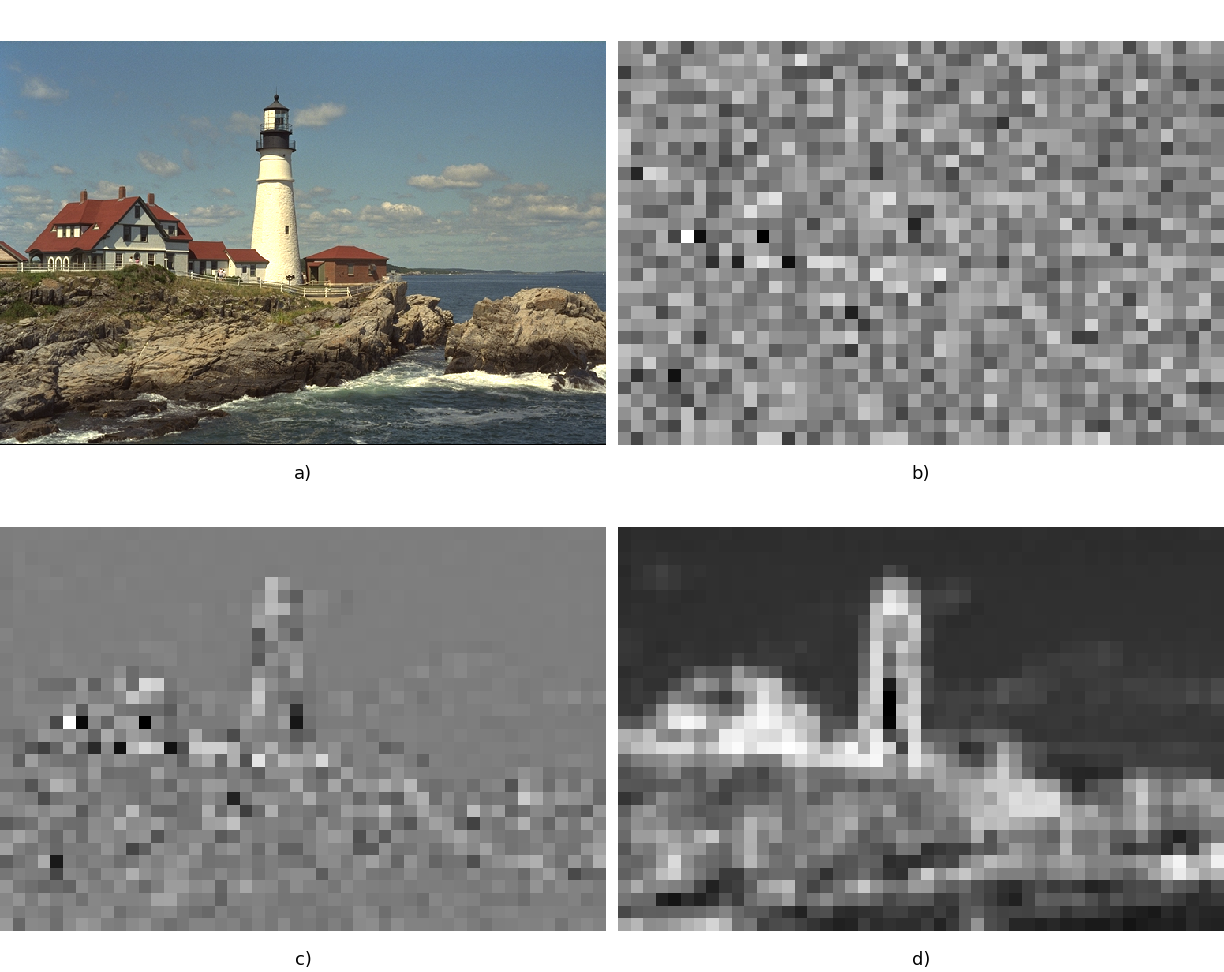
\includegraphics[width=\textwidth]{../img/plots/vae_latents/vae_rand_posterior}
  \caption{\textbf{a)} \texttt{kodim21.png} from the Kodak Dataset. \textbf{b)}
    A random sample from the VAE posterior. \textbf{c)} Posterior means in a
  randomly selected channel. \textbf{d)} Posterior standard deviations in the same
  randomly selected channel. We can see that there is a lot of structure in the
  latent space, on which the full indepenence assumption will have a detrimental
  effect. (We have examined several random channels and observed the
  similarly high structure. We present the above cross-section without preference.)}
  \label{fig:vae_rand_posterior}
\end{figure}

\paragraph{Data Likelihood and Training Objective}
As is standard for VAEs, we aim to maximize the the (weighted) Evidence
Lower Bound (ELBO):
\begin{equation}
\label{eq:regular_vae_elbo}
\Exp_{q^{(1)}}[\log p(\vec{x} \mid \vec{z}^{(1)})] - \beta\KL{q^{(1)}}{p^{(1)}}.
\end{equation}
As the latent posterior and prior are both Gaussians, the KL can be computed
analytically, and there is no need for a Monte Carlo estimation. A popular and
simple choice for the likelihood to be chosen a Gaussian, in which case the
expectectation of the log-likelihood corresponds to the mean squared error
between the original image and its reconstruction. This also corresponds to
optimizing for the PSNR as the perceptual metric. However, it has been shown
that PSNR correlates badly with the HVS's perception of image quality \cite{girod1993s}
\cite{eskicioglu1994image}. This is mainly because an MSE training objective is
tolerant to small deviations regardless of the structure in the image, and hence
this leads to blurry colour patch artifacts in low-textured regions, which the
HVS quickly picks up as unpleasant. A thorough survey of different
training objectives for image reconstruction was performed by
\cite{zhao2015loss}. As far as we are aware, they were also the first to propose
MS-SSIM as a training objective as well. However, they also show another
interesting result: Mean Absolute Error (MAE) already significantly reduces and
in some cases completely removes the unpleasant artifacts introduced by MSE.
This is because MAE no longer underestimates small deviations, at the cost of
somewhat blurrier edges, which MSE penalized more. The MAE corresponds to a
diagonal Laplacian log-likelihood with unit scale, which is what we ended up
using. This results in
efficient training (an MS-SSIM training loss is very expensive to compute) as
well as it will enable us for a further enchancement, see Section
\ref{sec:learn_gamma}.

Concretely, our likelihood is going to be
\begin{equation}
\label{eq:laplace_likelihood}
  p(\vec{x} \mid \vec{z}^{(1)}) = \Laplace{\vec{\hat{x}} \mid
  \MU^{d, (1)}(\vec{\tilde{z}}^{(1)}), I},
\end{equation}
where $\MU^{d, (1)}$ is the reverse operation of $\MU^{e, (1)}$.


\subsubsection{Probabilistic Ladder Network}
\label{sec:prob_ladder_networks}

\begin{figure}
  \centering
  \includegraphics[width=\textwidth]{../img/thesis/VAE_architecture}
  \caption{PLN network architecture. The blocks signal data transformations, the
    arrows signal the flow of information. \textbf{Block descriptions:}
    \textit{Conv2D:} 2D convolutions along the spatial dimensions, where the
    $W\times H \times C / S$ implies a $W \times H$ convolution kernel, with $C$
  target channels and $S$ gives the downsampling rate (given a preceding letter
  ``d'') or the upsampling rate (given a preceding letter ``u''). If the slash
  is missing, it means that there is no up/downsampling. All convolutions operate
  in \texttt{same} mode with mirror padding. \textit{GDN / IGDN:} these are the
  non-linearities described in \cite{balle2016end}. \textit{Leaky ReLU:}
  elementwise non-linearity defined as $\max\{x, \alpha x\}$, where we set
  $\alpha=0.2$. \textit{Sigmoid:} Elementwise non-linearity defined as
  $\frac{1}{1 + \exp\{-x\}}$. We ran all
  experiments presented here with $N = 196, M = 128, F = 128, G = 24$.}
  \label{fig:pln_architecture}
\end{figure}

\par
As mentioned in \cite{balle2018variational}, their scale hyperprior architecture
closely resembles a \textit{probabilistic ladder network} (PLN), as defined by
\cite{sonderby2016train}. We quickly present here a brief overview of them.
\par
In order to understand PLNs, we start by a slightly simpler model family:
hieararchical VAEs (H-VAEs). For simplicity's sake, we consider two stochastic
level H-VAEs and PLNs only, the ideas here extend trivially to more stochastic levels.
On a basic level, we will be merely just stacking VAEs on top of each other.
Hence, for reference we define level 0 as the input - output layer pairs. The
\par
To get a 2-level H-VAE, once $\vec{\tilde{z}}^{(1)}$ is sampled, we use it to predict
the statistics of the second level posterior
\[
  q^{(2)}(\vec{z}^{(2)} \mid \vec{z}^{(1)}) = \Norm{\vec{z}^{(2)} \mid 
  \MU^{e, (2)}(\vec{\tilde{z}}^{(1)}), \SIGMA^{e, (2)}(\vec{\tilde{z}}^{(1)})},
\]
where $\MU^{e, (2)}(\vec{\tilde{z}}^{(1)})$ and
$\SIGMA^{e, (2)}(\vec{\tilde{z}}^{(1)})$ are analogous to their first level
counterparts. Next the second level is sampled $\vec{\tilde{z}}^{(2)} \sim
q^{(2)}$. The second level prior $p^{(2)}(\vec{z}^{(2)})$ is now the diagonal
unit-variance Gaussian, and the first level priors' statistics are predicted
using $\vec{\tilde{z}}^{(2)}$:
\[
  p^{(1)}(\vec{z}^{(1)} \mid \vec{z}^{(2)}) =
  \Norm{\vec{z}^{(1)} \mid \MU^{d, (2)}(\vec{\tilde{z}}^{(2)}),
    \SIGMA^{e, (2)}(\vec{\tilde{z}}^{(2)})}.
\] 
The data likelihood's mean is predicted using $\vec{\tilde{z}}^{(1)}$ as before
\cite{sonderby2016train}.
\par
The issue with H-VAEs is that the flow of information is limited by the
bottleneck of the final stochastic layer. PLNs resolve this issue by allowing
the flow of information between lower levels as well. To arrive at them, we
make the following modification to our H-VAE: first, once $q^{(1)}$ is known,
instead of sampling it immediately, we instead use its mean to predict the
statistics of the second level posterior:
\[
  q^{(2)}(\vec{z}^{(2)} \mid \vec{z}^{(1)}) = \Norm{\vec{z}^{(2)} \mid 
  \MU^{e, (2)}(\MU_{\vec{x}}), \SIGMA^{e, (2)}(\MU_{\vec{x}})},
\]
where $\MU_{\vec{x}} = \MU^{e, (1)}(\vec{x})$. Now, $\vec{\tilde{z}}^{(2)} \sim
q^{(2)}$ is sampled. The first level prior $p^{(1)}$ is calculated as before.
Finally, we allow the flow information on the first level by combining $q^{(1)}$
and $p^{(1)}$, inspired by the self-conjugacy of the Normal distribution in
Bayesian inference\footnotemark:
\[
  q^{(1)}(\vec{\tilde{z}}^{(1)} \mid \vec{\tilde{z}}^{2}, \vec{x}) =
  \Norm{\vec{\tilde{z}}^{(1)} \,\bigg|\,
    \frac{\SIGMA_{\vec{z}^{(1)}}^{-1} \MU_{\vec{x}} + \SIGMA_{\vec{x}}^{-1}
      \MU_{\vec{z}^{(1)}}}{\SIGMA_{\vec{x}}^{-1} + \SIGMA_{\vec{z}^{(1)}}^{-1}
    },
  \frac{1}{\SIGMA_{\vec{x}}^{-1} + \SIGMA_{\vec{z}^{(1)}}^{-1} }}
\]
We sample $\vec{\tilde{z}}^{(1)} \sim q^{(1)}(\vec{\tilde{z}}^{(1)} \mid
\vec{\tilde{z}}^{2}, \vec{x})$, and predict the mean of the likelihood using it.
\par 
The reason why H-VAEs and PLNs are more powerful models than regular VAEs, is
because regular VAEs make an independence assumption between the latents to make
the model tractable to compute, while H-VAEs and PLNs relax this assumption to a
\textit{conditional indpendence} assumption. This is the same way
\cite{balle2018variational}.
\footnotetext{We note that the formula we used is the actual combination rule
  for a Gaussian likelihood and Gaussian prior. The formula given in
  \cite{sonderby2016train} is slightly different. We are not sure if it is a
  typo or it is what they actually used. We found our combination rule worked
  quite well in practice.}

\begin{figure}
  \centering
  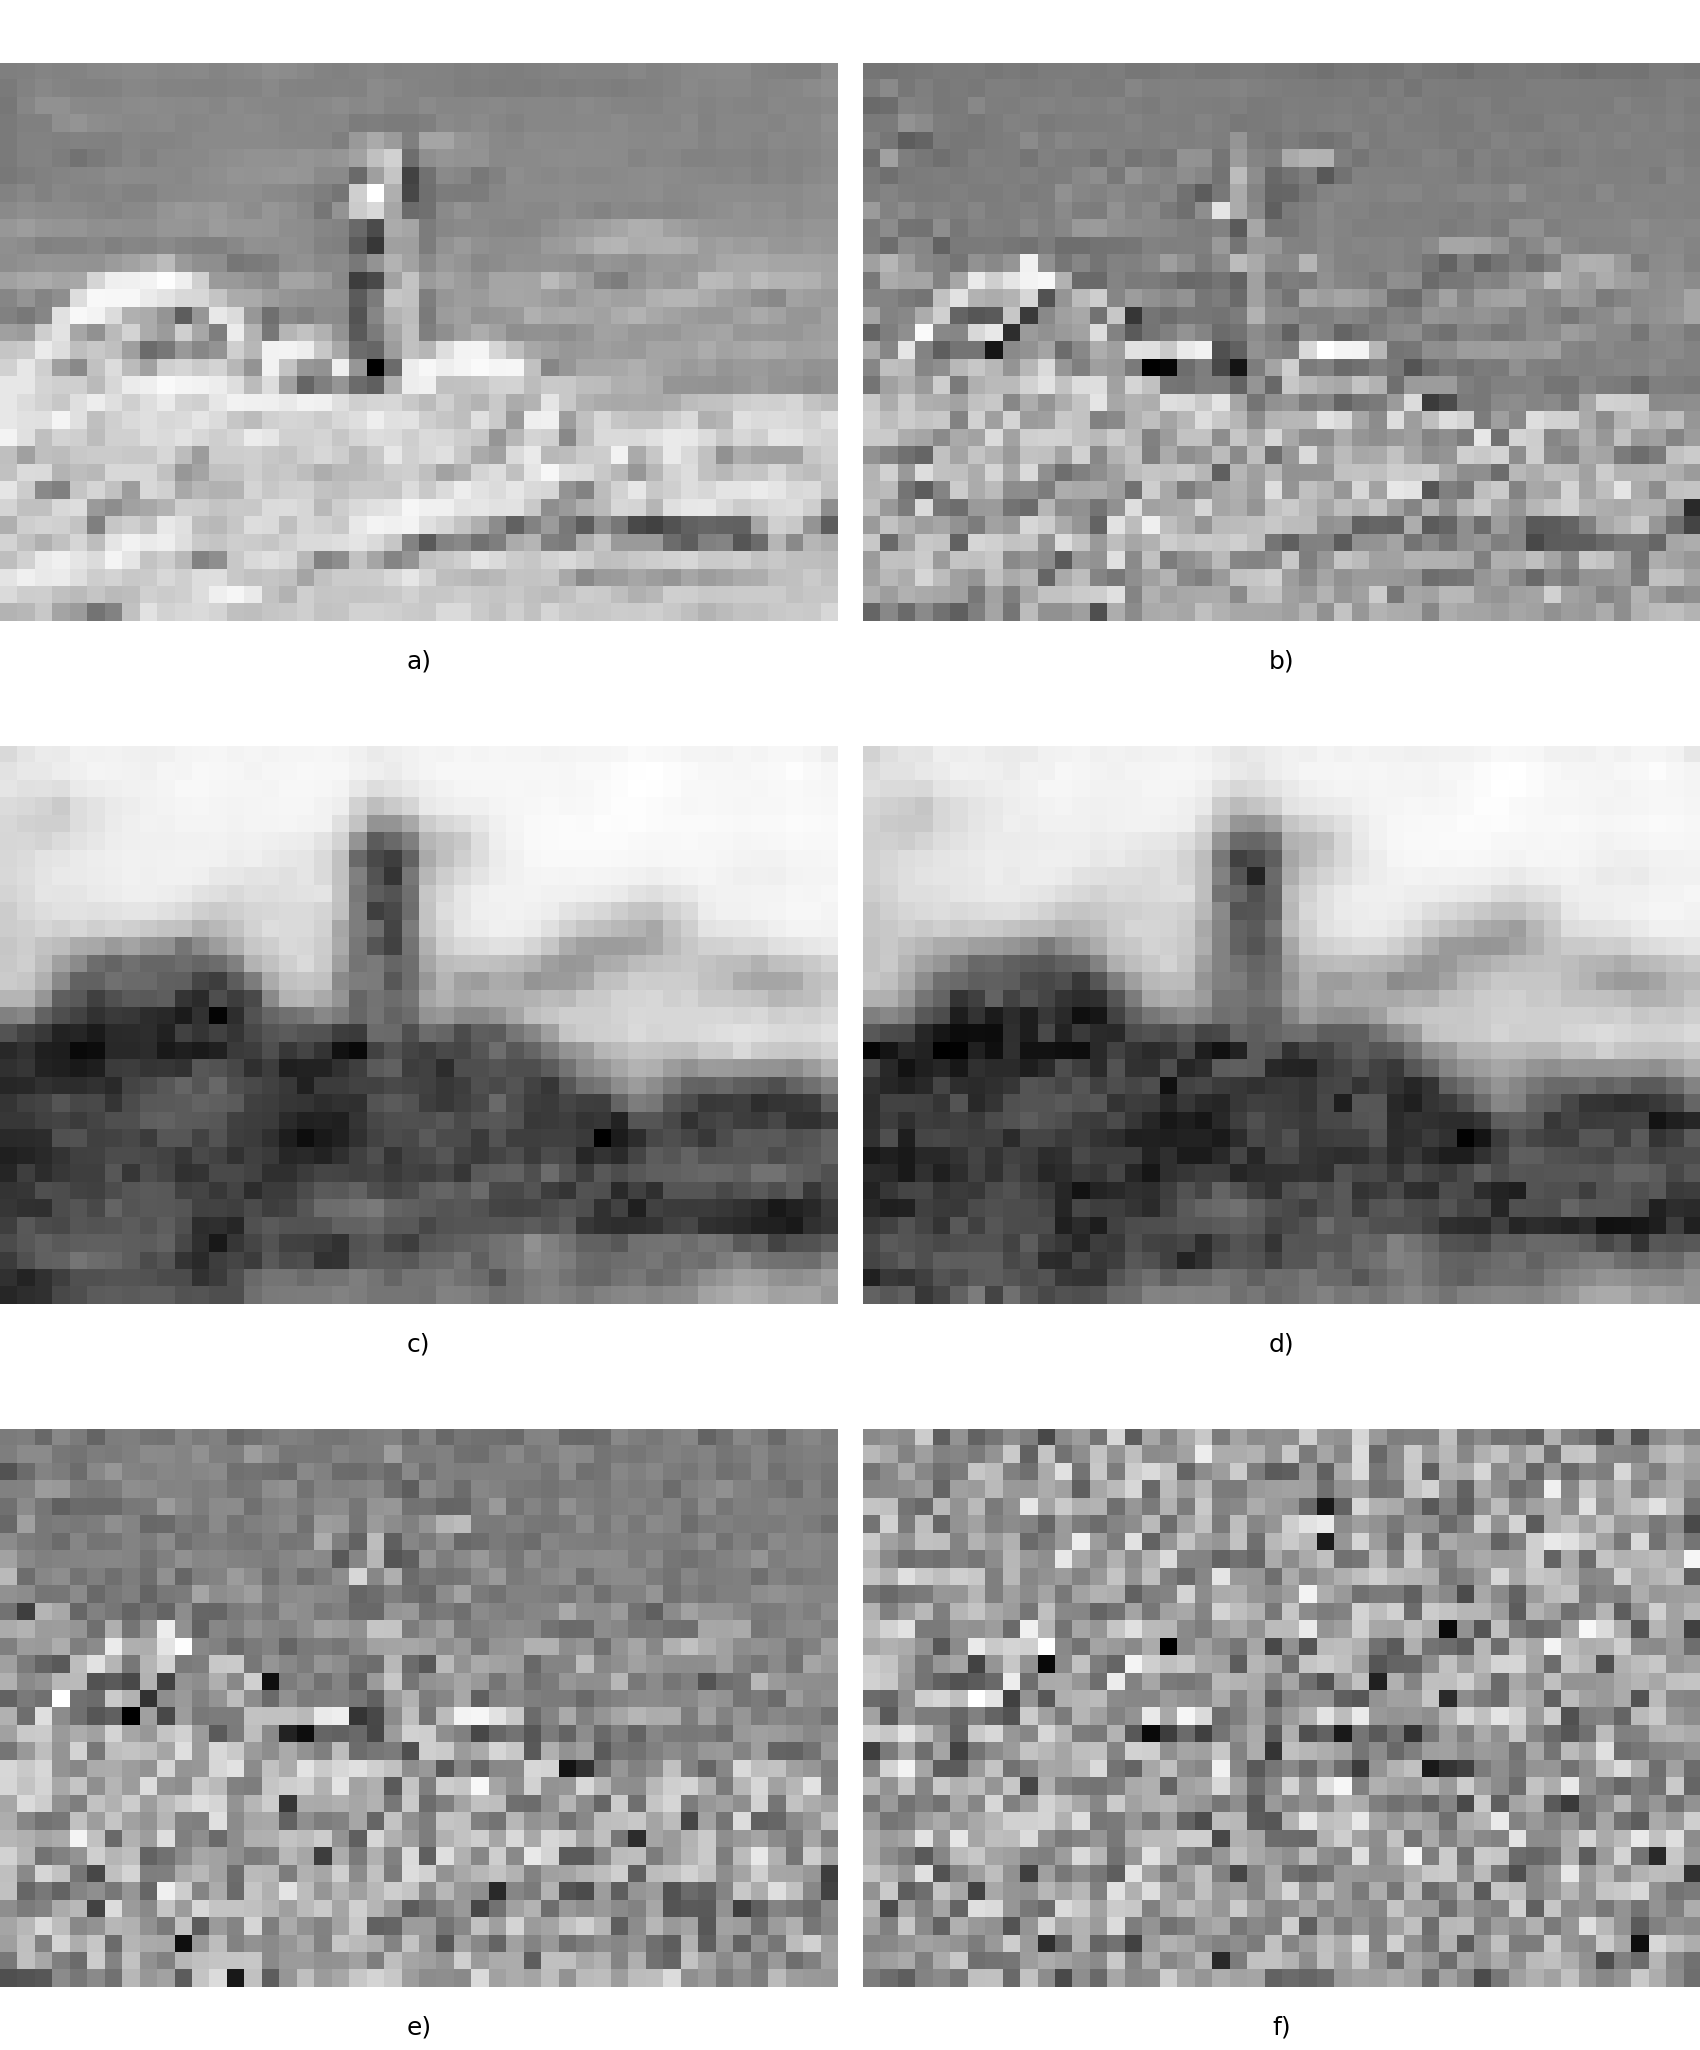
\includegraphics[width=\textwidth]{../img/plots/vae_latents/ladder_rand_posterior}
  \caption{We continue the analysis of the latent spaces induced by
    \texttt{kodim21} from the Kodak Dataset. Akin to Figure
    \ref{fig:vae_rand_posterior}, we have selected a random channel for both the
    first and second levels each and present the spatial cross-sections along these
    channels. \textbf{a)} Level 1 prior means. \textbf{b)} Level 1 posterior means.
    \textbf{c)} Level 1 prior standard deviations. \textbf{d)} Level 1 posterior
    standard deviations. \textbf{e)} Random sample from the Level 1 posterior.
    \textbf{f)} The sample from \textbf{e)} standardized according to the level
    1 prior. Most structure from the sample is removed, hence we see that the
    second level has successfully learned a lot of the dependencies between the
    latents. We have checked cross-sections along several randomly selected
    channels and observed the same phenomenon. We present the above with no preference.}
  \label{fig:ladder_rand_posterior}
\end{figure}

\par
Finally we need to update the regularizing term of the ELBO to incorporate the
joint posterior and priors over the latents. Luckily, we can break it up as
\[
  \KL{q(\vec{z}^{(1)}, \vec{z}^{(2)} \mid \vec{x})}{p(\vec{z}^{(1)}, \vec{z}^{(2)})} = 
  \KL{q(\vec{z}^{(2)} \mid \vec{x})}{p(\vec{z}^{(2)})} + 
  \KL{q(\vec{z}^{(1)} \mid \vec{z}^{(2)} , \vec{x})}{p(\vec{z}^{(1)} \mid \vec{z}^{(2)})},
\]
which we can now compute analytically again.

\subsection{Training}
\par \cite{sonderby2016train} give two key advices on training PLNs:
\begin{itemize}
\item use batch normalization \cite{ioffe2015batch}
\item and use a warmup on the coefficient of the KL term in the loss.
  Concretely, given a target coefficient $\beta_0$, the actual coefficient they
  recommend should be
  \[
    \beta(t) = \min\left\{ \frac{t}{W}, 1 \right\} \times \beta_0,
  \]
  where $t$ is the number of current batch and $W$ is the \textit{warmup period}.
\end{itemize} 
We ended up not utilizing point 1, due to an argument of
\cite{balle2018variational}, namely that GDN already performs a similar kind of
normalization as BN, and in the same way as it did not impact their training
results, we did not expect it to do for us either.
\subsubsection{Learning the Variance of the Likelihood}
\label{sec:learn_gamma}
\par
As we have noted, the reconstructions are blurry.
A solution offered by \cite{dai2019diagnosing} is to introduce a new parameter
$\gamma$ to the model, that will be the scale of the data likelihood. In our
case, since we are using a Laplace likelihood, we will have
\[
  p(\vec{\hat{x}} \mid \vec{z}^{(1)}) = \Laplace{\vec{\hat{x}} \mid \MU^{d,
      (1)}(\vec{\tilde{z}}^{(1)}, \gamma)}.
\]
In the case of a Gaussian, $\gamma$ would be the variance of the distribution.
Then, it is suggested that instead of predicting gamma (i.e. using a
heteroscedastic model), or setting it as a hyperparameter, \textit{we learn it}.
In \cite{dai2019diagnosing} this is used in conjunction with another novel
technique to achieve generative results with VAEs that are competitive with
state-of-the-art GANs. In this work however, as the second technique is more
irrelevant to us, we focus on learning $\gamma$ only.
\par
Let us examine this concept a bit more: let $D$ be the (original) log-likelihood
term with unit scale, and $R$ the (original) regularizing term, already
multiplied by our target coefficient $\beta$. Then, our new loss is going to be
\[
  L = \frac{1}{\gamma}D + R.
\]
Multiplying this through by $\gamma$ does not change the minimizer of the
expression, but we get the new loss
\[
  L' = D + \gamma R.
\]
In \cite{dai2019diagnosing} it is shown that if $\gamma$ is learned, then it is
always true that $\gamma \rightarrow 0$ as $t \rightarrow \infty$. This means,
that if we set some target $\gamma_\infty$, and use
\[
  \gamma' = \max\{ \gamma, \gamma_\infty \},
\]
as the scale of the data likelihood, we actually get a dual effect to the warmup
recommended by \cite{sonderby2016train}, but the scaling is automatic!
\begin{figure}
  \centering
  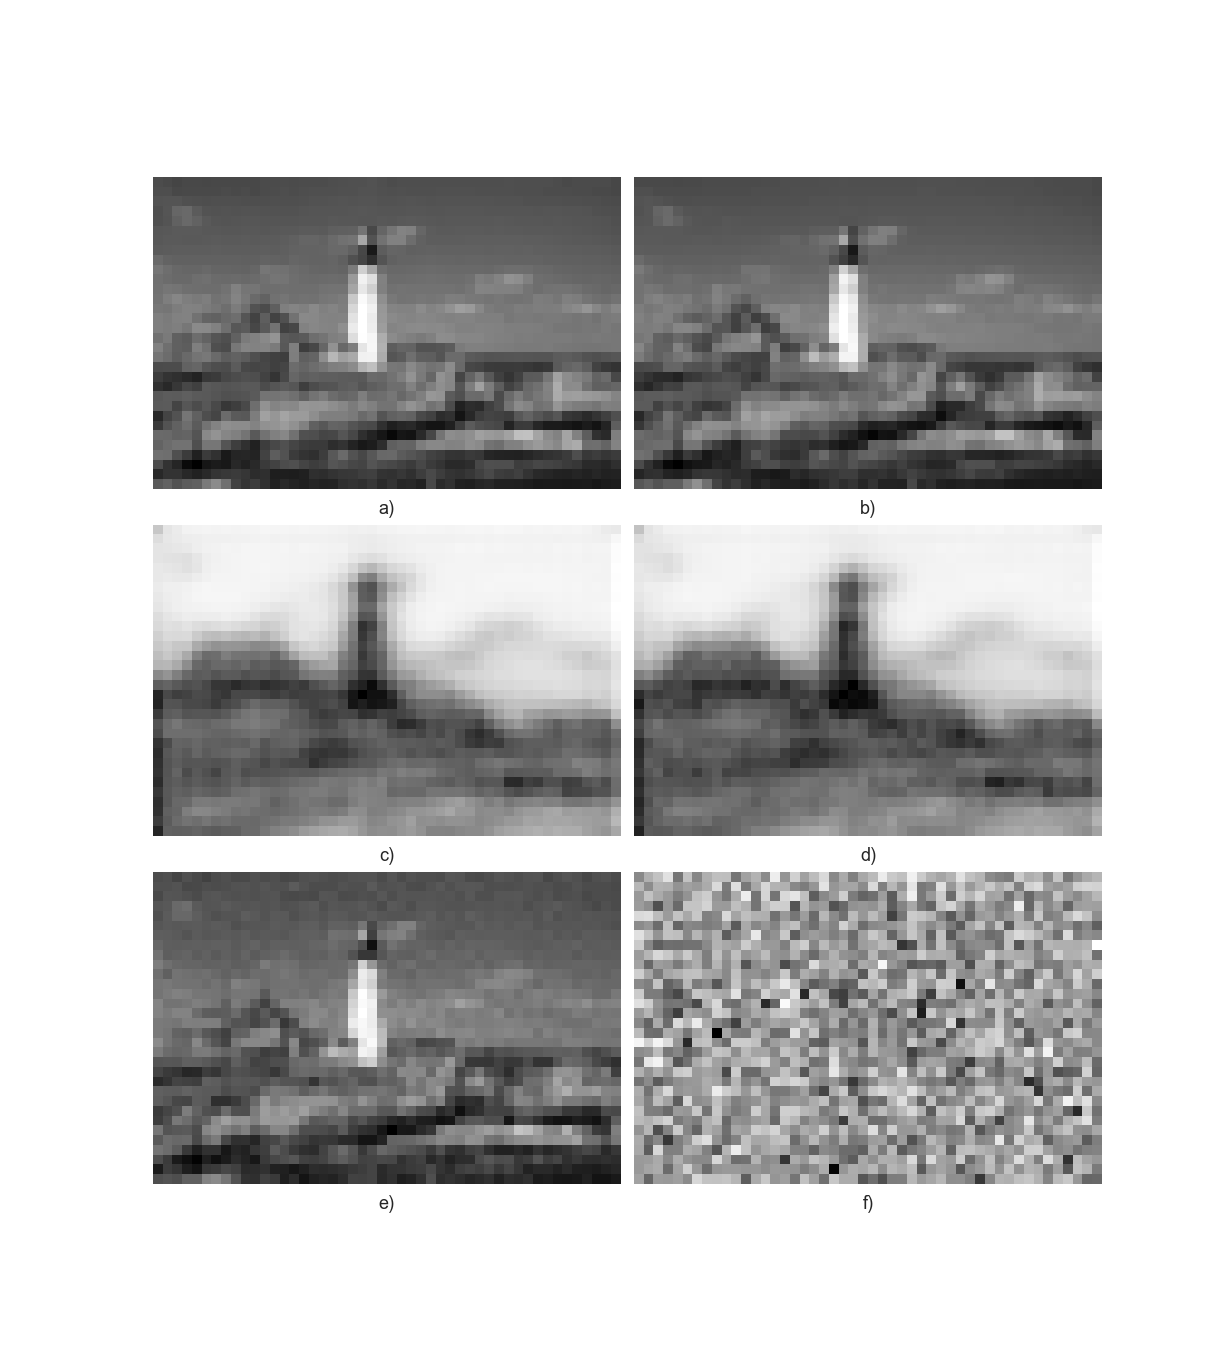
\includegraphics[width=\textwidth]{../img/plots/vae_latents/gamma_rand_posterior}
  \caption{We continue the analysis of the latent spaces induced by
    \texttt{kodim21} from the Kodak Dataset. Akin to Figures
    \ref{fig:vae_rand_posterior} and \ref{fig:ladder_rand_posterior},
    we have selected a random channel for both the
    first and second levels each and present the spatial cross-sections along these
    channels. \textbf{a)} Level 1 prior means. \textbf{b)} Level 1 posterior means.
    \textbf{c)} Level 1 prior standard deviations. \textbf{d)} Level 1 posterior
    standard deviations. \textbf{e)} Random sample from the Level 1 posterior.
    \textbf{f)} The sample from \textbf{e)} standardized according to the level
    1 prior. We observe the same phenomenon, with no significant difference, as
    in Figure \ref{fig:ladder_rand_posterior}. We note that while the posterior
    sample may seem like it has more significant structure than the one in the
    previous Figure. This is only coincidence; some of the regular PLN's
    channels contain similar structure, and some of the $\gamma$-PLN's channels
    contain more noisy elements.
  }
  \label{fig:gamma_rand_posterior}
\end{figure}

\subsection{Coded Sampling}
\label{sec:coded_sampling}
\par
Once the appropriate network has been trained, this means that for any image $\vec{x}$
we are able to produce a latent posterior $q(\vec{z} \mid \vec{x})$ and prior
$p(\vec{z})$. Hence, as alluded to in Section \ref{sec:miracle_theory}, we can
use the MIRACLE algorithm to code $\vec{x}$ in approximately $\KL{q}{p}$ nats!
The question is how MIRACLE can be adapted to our setting. There are several key
differences in our situation compared to the setting in
\cite{havasi2018minimal}:

\begin{itemize}
\item \textbf{Variable sized latent space:} The original method has been
  developed for compressing the weight distribution of a BNN, whose dimension is
  fixed. In our case, due to our fully convolutional architecture, our rendition
  of the algorithm must be able to adapt gracefully to a range of latent space
  dimensions which can be as much as 4 magnitudes different for each other.

\item \textbf{Different posterior effects:} as our latent spaces will carry much
  more information about the topological nature of the coded image, the
  distribution of informative versus non-informative posteriors, and their
  properties will be different from the original setting, and we will need to
  adapt to these effects.

\item \textbf{Practicality / Resource efficiency:} Since the original method has
  been proposed to compress neural networks after they have been trained, the
  algorithm was proposed with people who have sufficient resources to train them
  in mind. In particular, the original method incorporates several rounds of
  incremental retraining during compression to guarantee their efficiency, which
  might require several GPU hours to complete. As our aim in this work to
  present a practical, universal compression algorithm, we must also design our
  method with a much broader audience in mind. Though we still assume the
  presence of a GPU, our requirements and coding times are much less harsh than
  that of the original work.
\end{itemize}

In the rest of this section we present the ways we have attempted to address the
above points.

\subsubsection{Parallelized Rejection Sampling}
\par
Our initial goal was to perform parallelization in a way that preserves image
quality, i.e. draws exact samples and also achieves the postulated upper bound.
As mentioned earlier, the rejection sampling algorithm given in
\cite{harsha2007communication} achieves this, and hence it served as a good
baseline. As pointed out in \cite{havasi2018minimal}, however, this algorithm
quickly becomes intractable once we leave the univariate setting. Fortunately, as we
are working with (conditional) independence assumptions between the latents,
sampling each dimension exactly by itself and then aggregating them will also
give an exact multivariate sample.
\begin{algorithm}
  \caption{Parallelized, bit-budgeted rejection sampling}
  \label{alg:multivariate_rej_samp}
  \begin{algorithmic}
    \Procedure{Rej-Sampler}{$B, P, Q, \langle x_i \sim Q \mid i \in \Nats \rangle$}
    \State $D \gets \text{dim}(P)$
    \State $p_{d, 0}(x) \gets 0 \quad \forall x \in \X, \forall d = 1,\hdots D$.
    \State $p_{d, 0}^* \gets 0, \forall d = 1,\hdots D$.
    \State $A = \vec{0} \in \{0, 1\}^D$
    \Comment Keeps track of whether a dimension has been accepted or not

    \State $S = \vec{0} \in \Reals^D$
    \Comment Sample we are ``building''

    \State $I = -\vec{1} \in \Nats^D$
    \Comment MIRACLE index vector for each dimension

    \For{$i \gets 1, \hdots 2^B$}

    \For{$d \gets 1, \hdots D$}

    \If{$A_d = 1$}

    \State Skip

    \EndIf


    \State
    $\alpha_{d, i}(x) \gets \min{P_d(x) - p_{d, i - 1}(x), (1 - p_{d, i - 1}^*)Q_d(x)}\quad
    \forall x \in \X$

    \State $p_{d, i}(x) \gets p_{d, i - 1}(x) + \alpha_{d, i}(x)$
    
    \State $p_{d, i}^* \gets \sum_{x \in \X}p_{d, i}(x)$

    \State $\beta_{d, i}(x_i) \gets \frac{\alpha_{d, i}(x)}{(1 - p_{d, i}^*)Q_d(x)}$

    \State Draw $u \sim \Unif{0, 1}$

    \If{$u < \beta_{d, i}(x_i)$}

    \State $A_d \gets 1$
    \Comment Indicate we accepted the sample

    \State $S_d \gets x_i$
    \State $I_d \gets i$

    \EndIf
    
    \EndFor
    \EndFor

    \State\Return $I, S$
    \EndProcedure
  \end{algorithmic}
\end{algorithm}

\par
We modify Algorithm \ref{alg:harsha_rej_sampling} in two ways to make it more
efficient. While their algorithm is Las Vegas, i.e. it always gives the right
answer, but in random time, this can get very inefficient if we have a few
dimensions with very high KL. Instead, to circumvent this issue and fix the
runtime of the algorithm, by allocating a bit budget $B$ to each dimension, and
only allowing $2^B$ samples to be examined. If the sample is accepted within
these draws, then we carry on with their sample indices. The
dimensions where every sample was rejected, we sample from the true target,
and quantize the samples to 16 bits. We then communicate these quantized
samples. The concrete details can be seen in Algorithm
\ref{alg:multivariate_rej_samp}.

\paragraph{Issues} Sadly, sampling each dimension individually leads to an
$\Oh(1)$ cost per dimension, as we will produce an index for each dimension, as
opposed to one index for the whole multivariate distribution. In other words,
the length of the concatenated indices will be much longer than the single index
that would be produced by rejection sampling the whole distribution. In Section
\ref{sec:rej_samp_artihmetic_coding} we discuss how we reduced these costs using
arithmetic coding.

\subsubsection{Refinement: Greedy Sampling}
\begin{algorithm}
  \caption{Greedy sampler}
  \label{alg:greedy_sampler}
  \begin{algorithmic}
    \Procedure{Greedy-Sampler}{$K, B, \MU_p, \SIGMA_p^2, q, \langle s_1, \hdots s_k \rangle$}

    \State $\vec{\tilde{z}}_0 \gets \vec{0}$
    \Comment Initialize the sample

    \State $I = ()$
    \Comment Initialize the index set to an empty list
    \For{$k = 1, \hdots, K$}

    \State Draw $\vec{s}_{k, b} \sim \Norm{\frac{\MU_p}{K}, \frac{\SIGMA_p}{K}}
    \quad$ for $b = 1,\hdots,B$
    
    \State $\vec{c}_{k, b} = \vec{\tilde{z}}_{k - 1} + \vec{s}_{k, b}$

    \State $\vec{\tilde{z}}_k \gets \argmax_{\vec{c}_{k, b}} \left\{ \log q(\vec{c}_{k, b}) \right\}$
    \Comment Create new sample

    \State $i_k \gets \argmax_{b} \left\{ \log q(\vec{c}_{k, b}) \right\}$
    \Comment Store the index of the shard sample that we used

    \State Append $i_k$ to $I$.
    
    \EndFor

    \State \Return $\vec{\tilde{z}}_K, I$
    
    \EndProcedure
  \end{algorithmic}
\end{algorithm}
\par
To solve the issue of dimensionality, we would need a way to code the sample
from the whole multivariate distribution. One way of doing this, as we have
seen, was using the indpendence assumption of the latents and break it up per
dimension. But there is another way. The strategy will be to progressively ``build''
a reasonable sample from the posterior. A well known fact about Gaussian
distributed random variables is that they are closed under addition. Concretely,
if $X \sim \Norm(\mu_X, \sigma^2_X), Y \sim \Norm(\mu_Y, \sigma^2_Y)$, then
\[
  X + Y \sim \Norm(\mu_X + \mu_Y, \sigma_X^2 + \sigma_Y^2).
\]
Assuming that the normals are diagonal multivariate Gaussians, the extension of
the above to it is straight forward.
Using this simple fact, we may now do the following: pick an integer, $K$, that
we will call the number of shards. Then, given the prior $p(\vec{z}^{(1)} \mid
\MU, \SIGMA^2)$, we can break it up into $K$ equal shards $p_k\left(\vec{z}^{(1)}
\mid \frac{\MU}{K}, \frac{\SIGMA^2}{K}\right)$. Now, for each individual shard,
we may allocate a bit budget $B$. Then, we draw $2^B$ samples from each shard.
Note, if we assign a different, but preagreed sequence of random seeds to each
shard, then each sample can be coded in $B$ bits. Start with an initial sample
$\vec{\tilde{z}}_0 = \vec{0}$. Now, draw $2^B$ samples $\vec{s}_{1, b}$ from the
first shard $p_1$ and create ``candidate samples''$\vec{c}_{1, b} =
\vec{\tilde{z}}_0 + \vec{s}_{1, b}$ and calculate their log-likelihoods under the
target. Finally, set $\vec{\tilde{z}}_1 = \argmax_{\vec{c}_{1, b}}\log
q(\vec{c}_{1, b})$, and repeat until we reach $\vec{\tilde{z}}_K$, at which
point we return it. Then the returned vector will be approximately from the
target. More precisely, this is a ``guided'' random walk, where we bias the
trajectory towards the median of the distribution. The algorithm is described in
more detail in Algorithm \ref{alg:greedy_sampler}.
\paragraph{A note on implementation}
We note that empirically the greedy sampler is sensitive to small variances on
the priors. To ameliorate this, we standardize the prior, and scale the
posterior according to the standardization, i.e. we set 
\[
  q'(\vec{z} \mid \vec{x}) = \Norm{\vec{z} \bigg| \frac{\mu_q -
      \mu_p}{\sigma_p}, \frac{\sigma^2_{q}}{\sigma^2_{p}}},
\]
where $\mu_p, \sigma^2_p$ are the statistics of the original prior and $\mu_q,
\sigma^2_q$ are the statistics of the original posterior. We communicate the
approximate sample $\vec{z}'$ from $q'$ instead of $q$. This is not problematic, as
Gaussian distributed random variables are closed under linear transformations,
i.e. given $X \sim \Norm{m, s^2}$, we have
\[
  \alpha X + \beta = Y \sim \Norm{\alpha m + \beta, \alpha^2 s^2}.
\]
Hence, the decoder may recover an approximate sample from $q$, by calculating
$\vec{z} = \sigma_{p} \vec{z}' + \mu_{p}$.
\paragraph{Issues}
While the greedy sampler makes sampling efficient and tractable from the
posterior, it comes at the cost of reduced sample quality. In particular, it
gives blurrier images. This also means that if we use a PLN to compress an
image and we use the greedy technique to code the latents on the second level,
the first level priors' statistics derived from the biased sample will be off,
and $KL{q(\vec{z}^{(1)} \mid \vec{z}^{(2)}, \vec{x})}{p(\vec{z}^{(1)} \mid
  \vec{z}^{(2)})}$ will be higher. We have verified empirically, that while
using a biased sample on the second level does not degrade image quality
(possibly due to the noise tolerance of VAEs), it does significantly increase
the compression size (by a factor of $1.2 - 1.5$) of the first level, which is
very significant. This motivated the final sampling algorithm presented here,
only used on the second level of our PLNs.

\subsubsection{Second Refinement: Adaptive Importance Sampling}
\begin{algorithm}
  \caption{Adaptive Importance Sampler}
  \label{alg:adaptive_importance_sampler}
  \begin{algorithmic}
    \Procedure{Adaptive-Importance-Sampler}{$K, G, B, P, Q, \langle x_i \sim Q \mid i \in \Nats \rangle$}
    \State $\Gamma \gets ()$
    \Comment Group sizes
    \State $kl_i \gets \KL{Q_i}{P_i} \forall i = 1, \hdots N$
    \Comment Get KLs for each dimension
    \State $OI \gets $ \Call{Where}{$kl_i > K$}
    \Comment Outlier indices in the vector
    \State Sample $O \sim Q_{OI}$
    \State $\hat{O} \gets $ \Call{Quantize}{O}
    \State $Q' \gets Q_{\setminus OI}$
    \Comment Target distribution restricted to the dimensions defined by $OI$.
    \State $P' \gets P_{\setminus OI}$
    \Comment Remove outlier dimensions
    \State $\gamma \gets 0$
    \Comment Current group size
    \State $k \gets 0$
    \Comment Current group KL

    \For{$i \gets 1, \hdots \text{dim}(Q')$}

    \If{$k + kl_i > B$ or $\gamma + 1> G$}

    \State Append $\gamma$ to $\Gamma$
    \State $k \gets kl_i$
    \State $\gamma \gets 1$

    \Else

    \State $k \gets k + kl_i$
    \State $\gamma \gets \gamma + 1$

    \EndIf

    \EndFor

    \State Append $\gamma$ to $\Gamma$
    \Comment Append the last group size

    \State $S = ()$
    \Comment Importance samples for the groups
    \State $I = ()$
    \Comment MIRACLE sample indices
    \State $g \gets 0$
    \Comment Current group index

    \For{$\gamma$ in $\Gamma$}
    \Comment Now importance sample each group

    \State $idx, s \gets$ \Call{Importance-Sample}{$P_{g:g + \gamma}, Q_{g: g +
        \gamma}, \langle x_i \sim Q \mid i \in \Nats \rangle$}
    \State Append $idx$ to $I$
    \State Append $s$ to $S$

    \EndFor

    \State \Return I, S

    \EndProcedure
  \end{algorithmic}
\end{algorithm}
The adaptive importance sampler uses the importance sampler described in
Algorithm \ref{alg:miracle_imp_samp}. The idea is to use the block based
importance sampling, as proposed in \cite{havasi2018minimal}, however, unlike
them we allocate the block sizes dynamically. In particular, we set a bit
budget $B$ per group, a maximum group size $G$ and an individual limit $K$.
We first begin by discarding individual dimensions where the KL is larger
than $K$. Then, we flatten the remaining dimensions in raster-scan order and 
iteratively add dimensions into the current group so long as the total KL of the
group reaches either the bit budget $B$ or the number of dimensions added to the
group reaches $G$. At this point we start with a new group. Once the whole
vector has been partitioned, we importance sample each group using Algorithm 
\ref{alg:miracle_imp_samp}. The removed dimensions are sampled directly from
the posterior and then the samples are quantized to 16 bits. The complete
algorithm can be seen in Algorithm \ref{alg:adaptive_importance_sampler}.
\par
For ease of referral, since we would perform Adaptive Importance Sampling on the
second level, followed by the Greedy Sampling on the first, We will refer to
this way of sample coding as IS-GS.
\subsection{Coding}
\label{sec:entropy_coding}
\par

\subsubsection{Coding the rejection sampled latents}
\label{sec:rej_samp_artihmetic_coding}
% why doesnt rejection sampling work exactly?
% - the cost is not arising from bad independence assumptions, because we have
%   indepenedence
% - so does it come from a bad match of the actual image posteriors?

\par
Simply writing the indices of the individual dimensions given by the rejection
sampler would be very inefficient, because without additional assumptions the
way to uniquely decode them would be to block code them (i.e. code all indices
in 8 bits, say). This would however would add an $\Oh(1)$ cost per dimension on
the coding length, which is very undesirable. Hence, we implemented a simple
non-adaptive arithmetic coder \cite{rissanen1981universal} to compress the 
indices even further. The
probabilities for the symbol table have been estimated  by encoding the entire
training set and using the empirical probability distribution. For unseen
indices we used Laplace smoothing. In particular, given the empirical
distribution of the sample indices $P$, the probability distribution
used is
\[
  \tilde{P}(i) = \begin{cases}
    (1 - \alpha)P(i) & \text{if } i \in I \\
    \frac{\alpha}{N} & \text{otherwise}
    \end{cases}
\]
where $I$ is the allowed index set, in our case since we allocated $B = 8$ bits
for each individual dimension, $I = \{0, \hdots 255\}$. Since we quantized the
outliers to 16 bits, $N = 2^{16} - 2^{8}$. We found that choosing $\alpha
\approx 0.01$ worked reasonably well.
\subsubsection{A note on the Arithmetic Coder}
\par
While for small alphabets the naive implementation of the arithmetic coder is
very fast, the decoding time actually grows as $\Oh(|\A|)$ in the size of the
alphabet. In particular, decoding the arithmetic code of a reasonably large
image would take up to 30 minutes using the naive implementation. The
inefficiency is due to a bottleneck where we need to find in a partition of $[0,
1]$ into which partition the currently coded interval fits. In the naive
implementation this is simply determined using a linear search over the
partitions. This can be made more efficient by using height-balanced binary
search trees (BSTs). In particular, we need to find the least upper bounding
item in the BST for the given point, which can be done in $\Oh(\log_2|\A|)$.
Using this additional trick, we can decode large images' code in a few seconds.
In particular we implemented an AVL-tree to serve as the BST, which is always
guaranteed to be height balanced \cite{adel1962algorithm}.
\subsubsection{Coding the greedy \& importance sampled latents}
\par
\paragraph{Importance Sampler}  For the importance sampler, we note that the
inefficiency of block coding the sample index goes away, as the $\Oh(1)$ cost is
now shared across the dimensions and is going to negligible, as well as
estimating empirical probabilities for indices would have been very costly and
would not have increased efficiency significantly. On the other hand, we also
have to communicate the groups as well. We note, that instead of communicating
group indices, we can instead order the latents and communicate consecutive
group sizes, from which the indices can be easily reconstructed, but each
group's size takes up at most $\lceil \log_2G \rceil$ bits. We also note that in
the best case we will have $\lceil \frac{N_2}{G} \rceil$ groups, but probably
more (where $N_2$ is the dimensionality of the second level). This means that
there is still a huge inefficiency here still, however so long as $N_2$ is
sufficiently small, compared to the codelength for the indices, it will be
manageable. We also note that the group size is likely to be biased towards
higher values, and hence building an empyrical distribution them and arithmetic
coding the sequence could lead to a big reduction in the inefficiency, however,
we found this not to be too important to focus on. 
\paragraph{Greedy Sampler} It is easy to see that the greedy sampler is already
as efficient as it could be. The sample indices for each shard are as compactly
represented, as we expect the maximum of the samples to be uniformly
distributed. Hence, the only other things that needs to be coded is the number
of shards and the number of samples for each shard for the cumulative sample to
be decodable. Hence, for the greedy sampler we just wrote the indices straight
to the binary file.

\section{Results}
\label{sec:experimental_results}
\par
In this section we detail how we setup and empiricall show the correctness and
the efficiency of our model. We compare our results against JPEG, the most
widely used lossy compression method \cite{bull2014communicating}, and the
current state-of-the-art, the results of \cite{balle2018variational}\footnotemark.
\cite{zhao2015loss}

\footnotetext{We thank the authors of the paper for making their data available
  to us.}

\paragraph{Note:} All experiments were run on a GeForce GTX 1080 GPU.

\subsection{Experimental Setup}
\par
As we based our models on that of \cite{balle2016end} and
\cite{balle2018variational}, we mirror a lot of their training setup as well
(See Section \ref{sec:dataset_preproc} for the dataset and preprocessing). We
trained all our models with Adam with a starting learning rate of $\alpha_0 =
3 \times 10^{-5}$ and trained all of our models for 20 epochs or equivalently,
approximately 200,000 iterations.. We used a smooth
exponential learning rate decay schedule except in the case of the
$\gamma$-VAEs, according to the formula
\[
  \alpha(t) = \alpha_0 \times r^{\frac{t}{D}}.
\]
Where $r$ is the decay rate, $D$ is the decay step size and $t$ is the current
batch number. We found $r = 0.96$ and $D = 1500$ worked well for our
experiments. We note, however, that we did not notice signifcant performance
gains by using this schedule compared to just using a fixed one.
\par
A surprising result is that even though we have not trained our models for
nearly as long, or on nearly as much data as \cite{balle2018variational}, our
method still gets reasonably close to their results. We compare our results to
theirs, which as far as we are aware are the current state-of-the-art on both
the MS-SSIM and PSNR perceptual metrics.

\subsection{Comparison of our method with other algorithms}
\par

We present the rate-distorsion curves for the following:
\begin{itemize}
\item JPEG, with quality settings from 1 to 92, with increments of 7 between
  settings. As this is the most widely used lossy image compression codec, it is
  crucial to demonstrate that our method is at least competitive with it, and
  ideally beats it.
\item BPG\footnotemark with 4:4:4 chroma sampling, as we are comparing against
  RGB-based compression techniques. We used quantization settings between 51 to
  33 wiht decrements of 3 between settings.
\item Two models with the same architecture from \cite{balle2018variational},
  one optimized for a MSE training objective, and one optimized for the
  MS-SSIM perceptual metric.
\item Two of our models, all of which were optimized with Laplacian likelihoods,
  one PLN and one $\gamma$-PLN. We plot both their theoretically optimal
  performance as well as their actual performance, with the differences
  explained below.
\end{itemize}

\par
For our method, for each model we present two results: the \textit{theoretically
optimal} performance, and the \textit{actual} performance. The theoretically
optimal BPP was calculated using the theoretically achievable upper bound for
the compression size in bits as given by \cite{harsha2007communication},
without the constant term:
\[
  \I[\vec{x} : \vec{z}] + 2 \log \left( \I[\vec{x} : \vec{z}] + 1\right).
\]
The optimal reconstruction error was calculated by passing an image through the
VAE regularly, instead of using the coded approximate sample. Thus, any
actual method's performance using the same setup must apper to the right of (less
efficient compression) or below (worse reconstruction quality) the theoretical
position.

\footnotetext{We used the implementation available at \url{http://bellard.org/bpg}}

We trained the PLNs using $\beta = \{0.01, 0.03, 0.1, 0.3, 1\}$ and the
$\gamma$-PLNs using $\beta = \{10, 3, 1, 0.3, 0.1\}$.

Our results can be seen in Figure \ref{fig:kodim01_comp}. We observe a similar
phenomenon as \cite{balle2018variational}: there is a mismatch in the comparison
of models according to different perceptual metrics, depending on what objective
they have been optimized for. In particular, JPEG and BPG have both been
optimized so that they give high PSNR (thus, low MSE), whereas they underperform
on the newer MS-SSIM metric. We note that as MS-SSIM correlates better with what
the HVS perceives, we find it more important to do well on that comparison.
\par
In interesting note, that also justifies our choice of the MAE as the training
objective, is the fact that our model optimized for it does well on this metric.

\begin{figure}
  \centering
  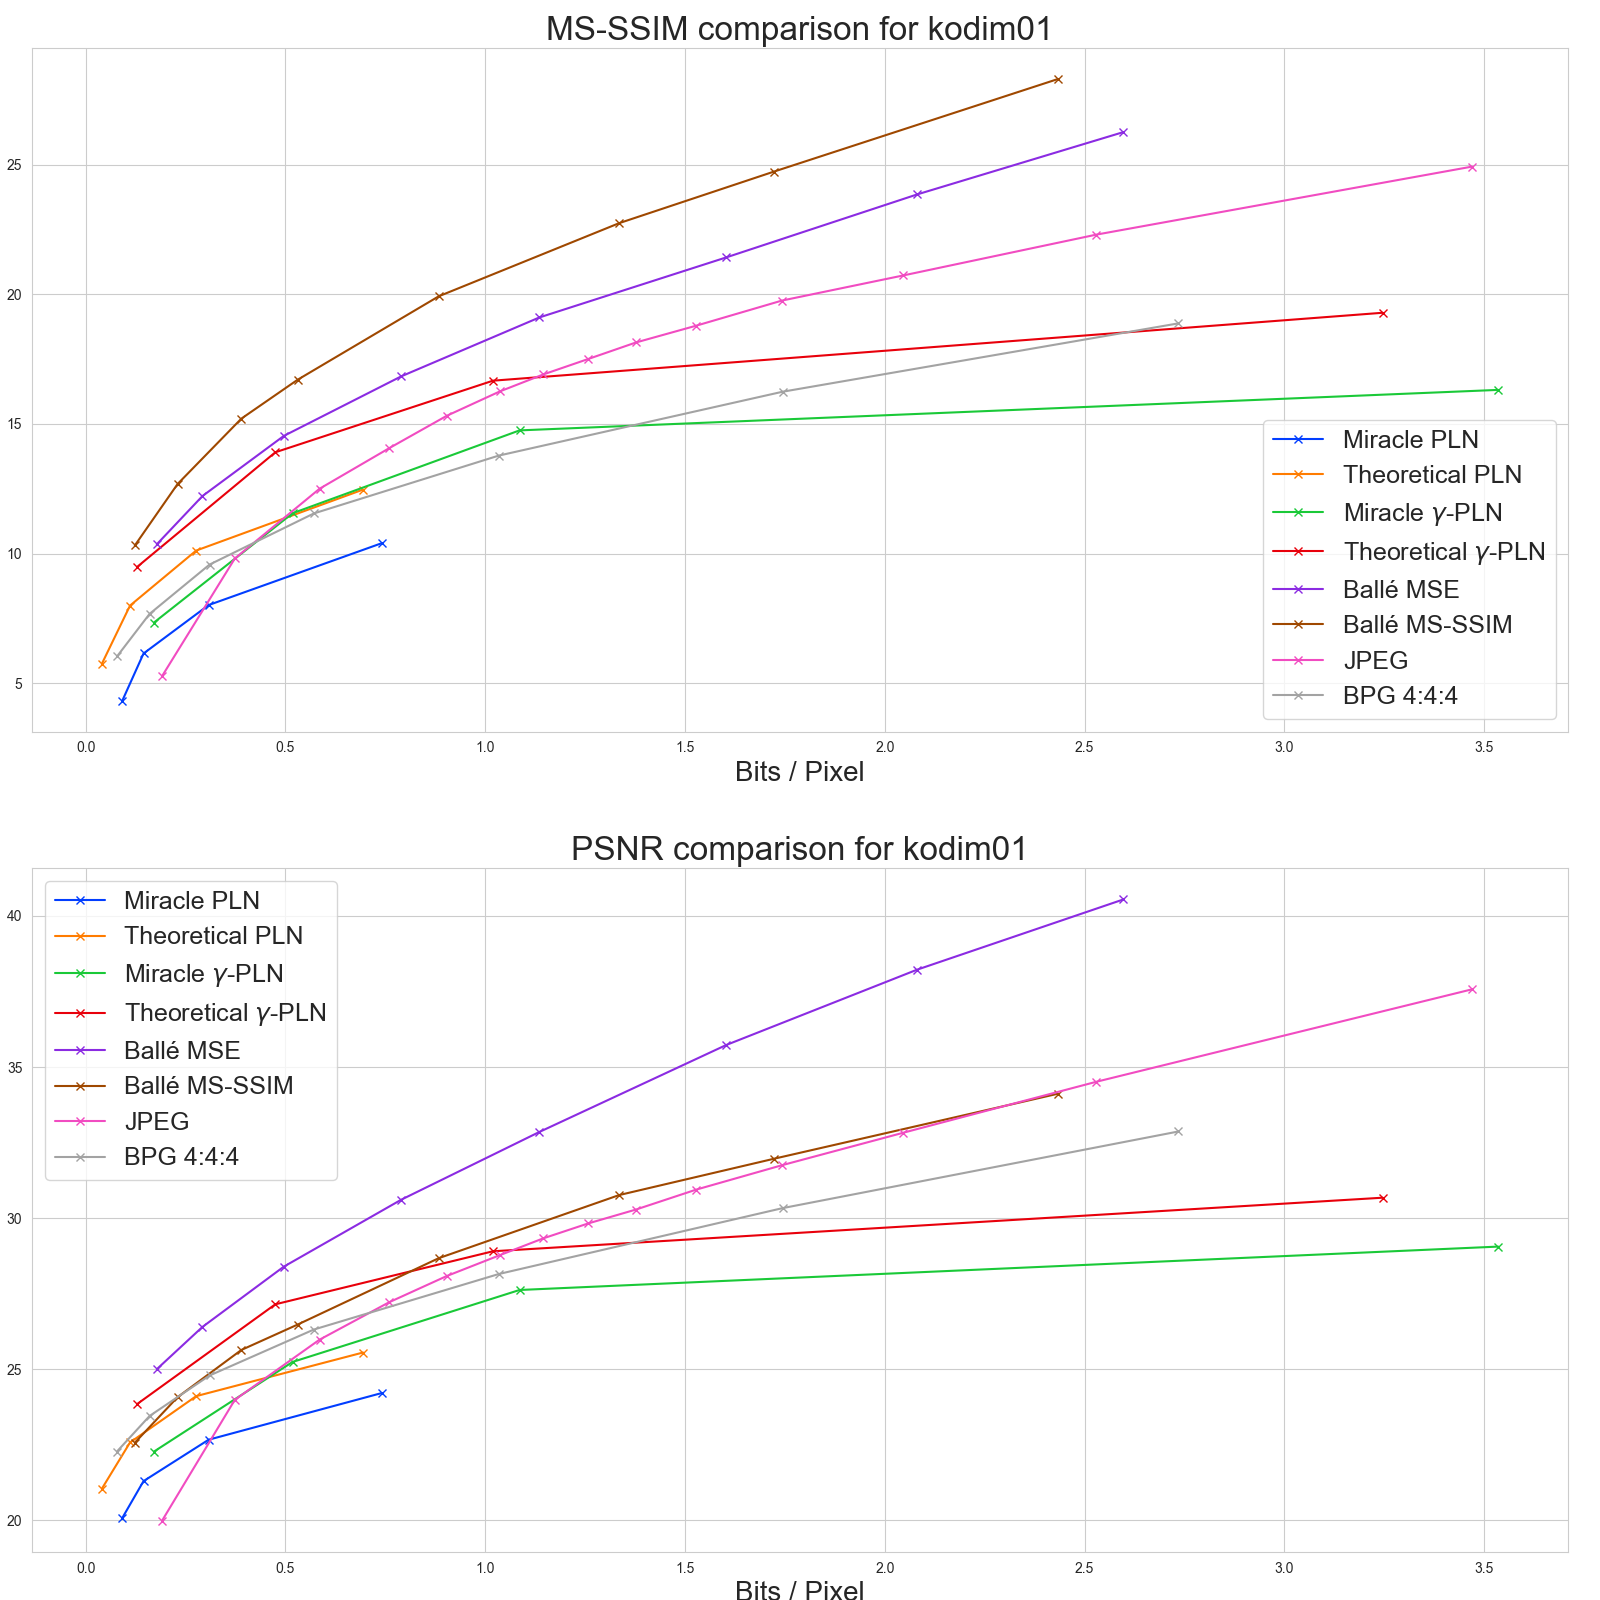
\includegraphics[width=\textwidth]{../img/plots/kodak_comparison/kodim01_comparison}
  \caption{Rate-Distorsion curves of several relevant methods. Please see
    Section \ref{sec:experimental_results} for the description of how we
    obtained each curve. We note that the MS-SSIM results are presented in
    decibels, where the conversion is done using the formula $-10 \cdot
    \log_{10}\left( 1 - \text{MS-SSIM}(\vec{x}, \vec{\hat{x}}) \right)$.
    The PSNR is computed from the mean squared error, using the formula 
    $-10 \cdot \log_{10}\text{MSE}(\vec{x}, \vec{\hat{x}})$.}
  \label{fig:kodim01_comp}
\end{figure}

\subsection{Analysis of the contribution of the second level}
\par
An important part of verifying the validity of using PLNs is to analyze the
contribution of the second level. Here we look at
\begin{itemize}
\item its contribution to the codelength
\item its efficiency in capturing dependencies between the first level latents
\end{itemize}

\begin{figure}
  \centering
  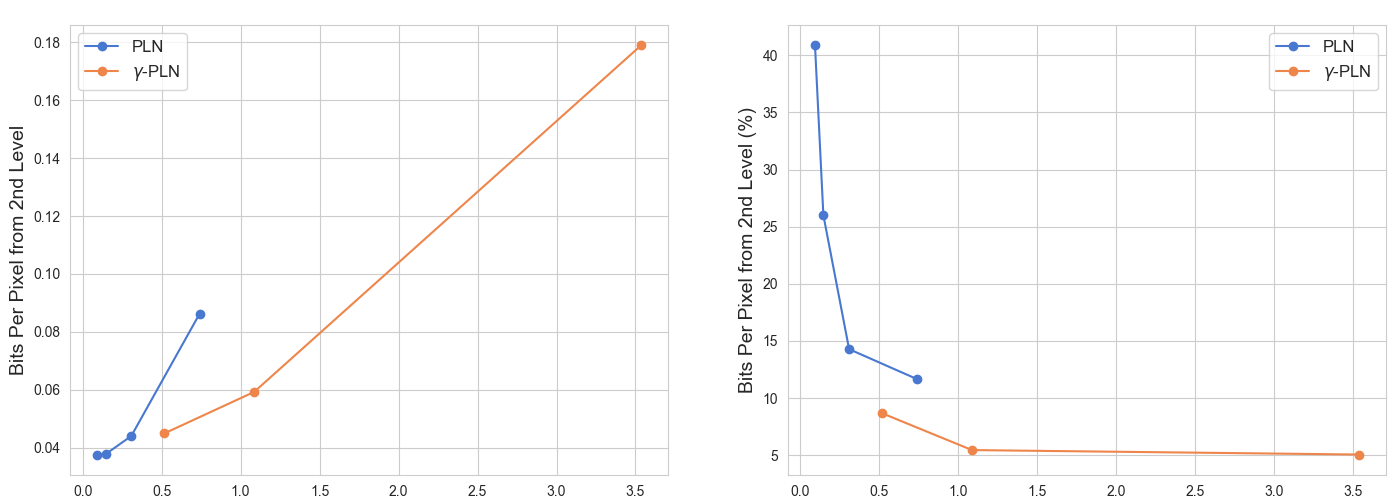
\includegraphics[width=\textwidth]{../img/plots/kodak_side_info/kodim01_side_info}
  \caption{Contribution of the second level to the rate, plotted agains the
    actual rate. \textbf{Left:} Contribution in BPP, \textbf{Right:}
    Contribution in percentages. We see that for lower bitrates there is more
    contribution from the second level and it quickly decreases for higher
    rates. It is also clear that on the same bitrates, the $\gamma$-PLN requires
    less contribution from the second level than regular PLN.}
  \label{fig:kodim01_side_info}
\end{figure}

\begin{figure}[H]
  \centering
  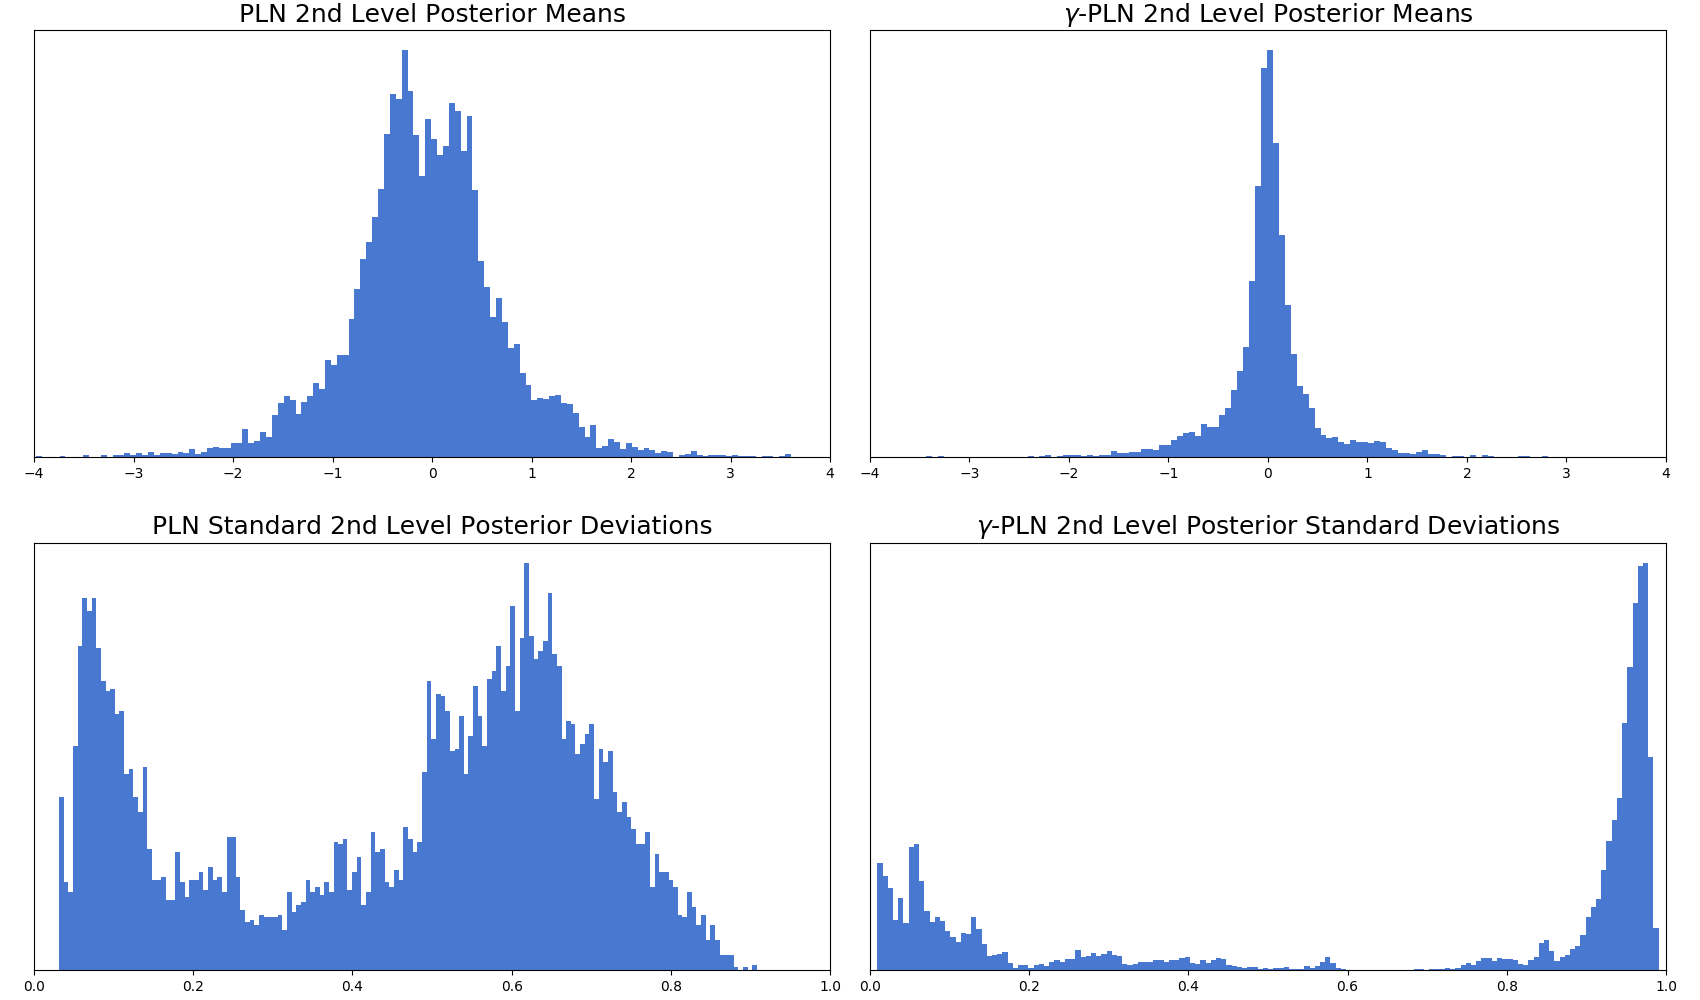
\includegraphics[width=\textwidth]{../img/plots/vae_latents/ladder_gamma_q2_comp}
  \caption{ladder on kodim21}
  \label{fig:ladder_gamma_q2_comp}
\end{figure}
\begin{figure}[H]
  \centering
  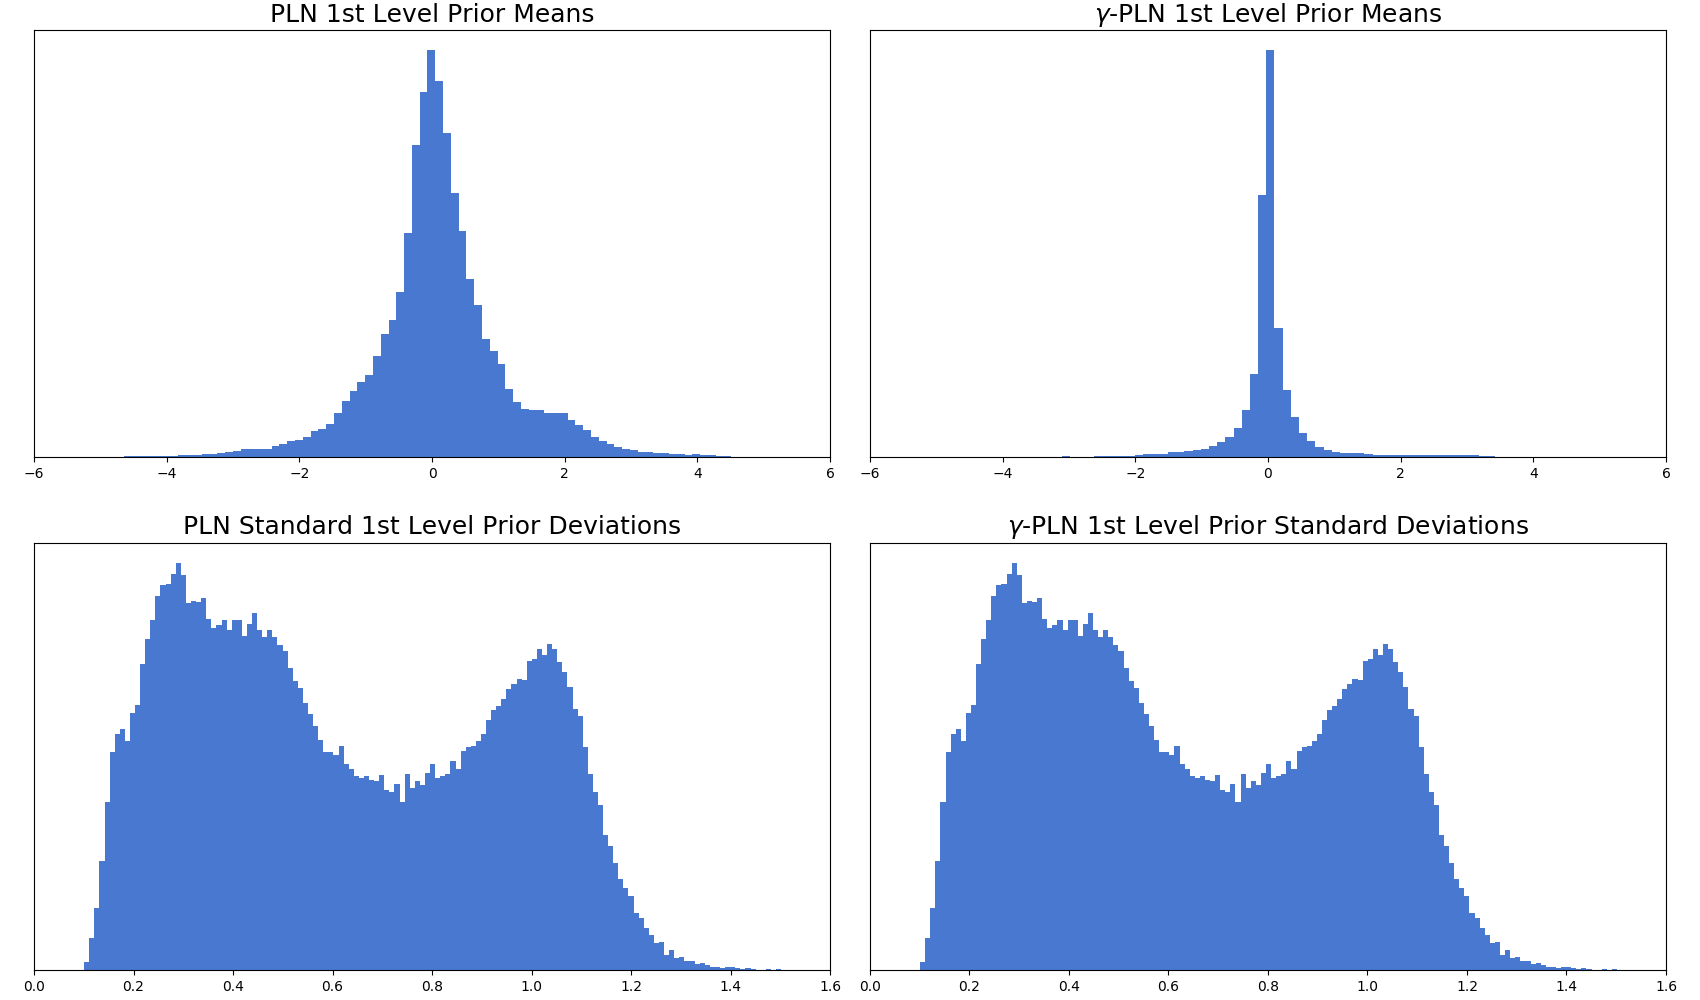
\includegraphics[width=\textwidth]{../img/plots/vae_latents/ladder_gamma_p1_comp}
  \caption{ladder on kodim21}
  \label{fig:ladder_gamma_p1_comp}
\end{figure}
\begin{figure}[H]
  \centering
  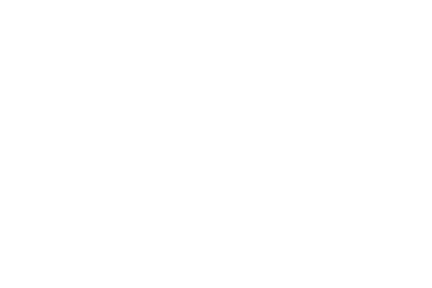
\includegraphics[width=\textwidth]{../img/plots/vae_latents/ladder_gamma_q1_comp}
  \caption{ladder on kodim21}
  \label{fig:ladder_gamma_q1_comp}
\end{figure}
\begin{figure}[H]
  \centering
  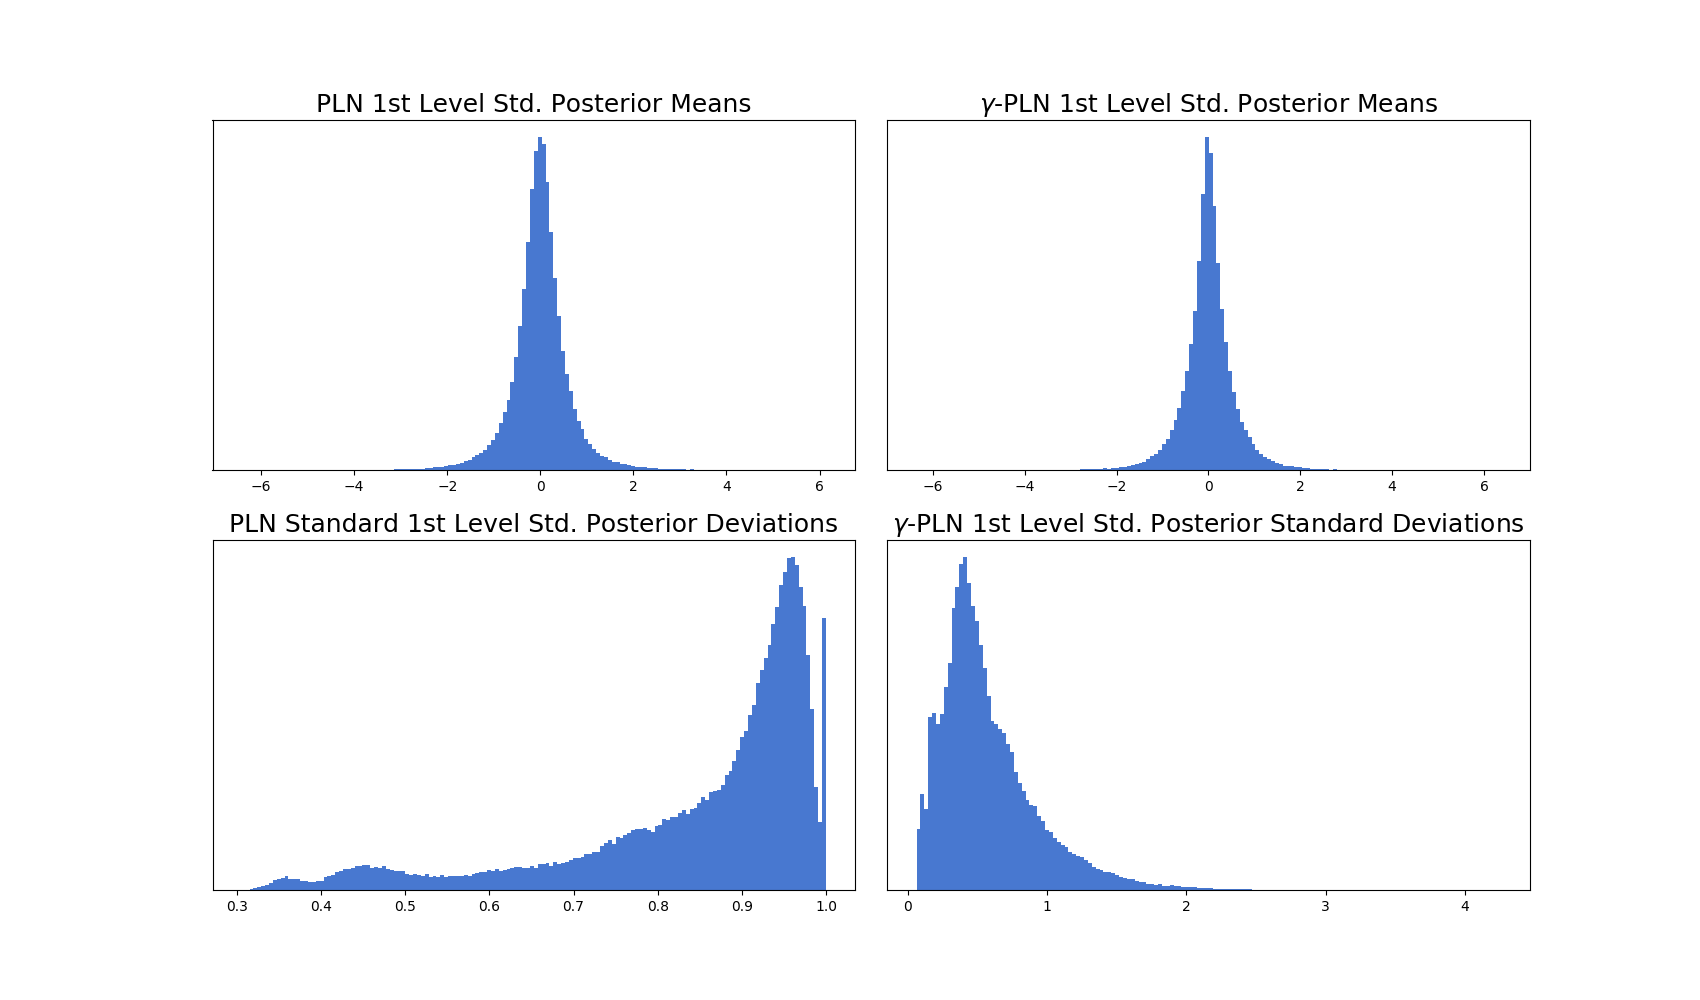
\includegraphics[width=\textwidth]{../img/plots/vae_latents/ladder_gamma_std_q1_comp}
  \caption{ladder on kodim21}
  \label{fig:ladder_gamma_std_q1_comp}
\end{figure}
\begin{figure}[H]
  \centering
  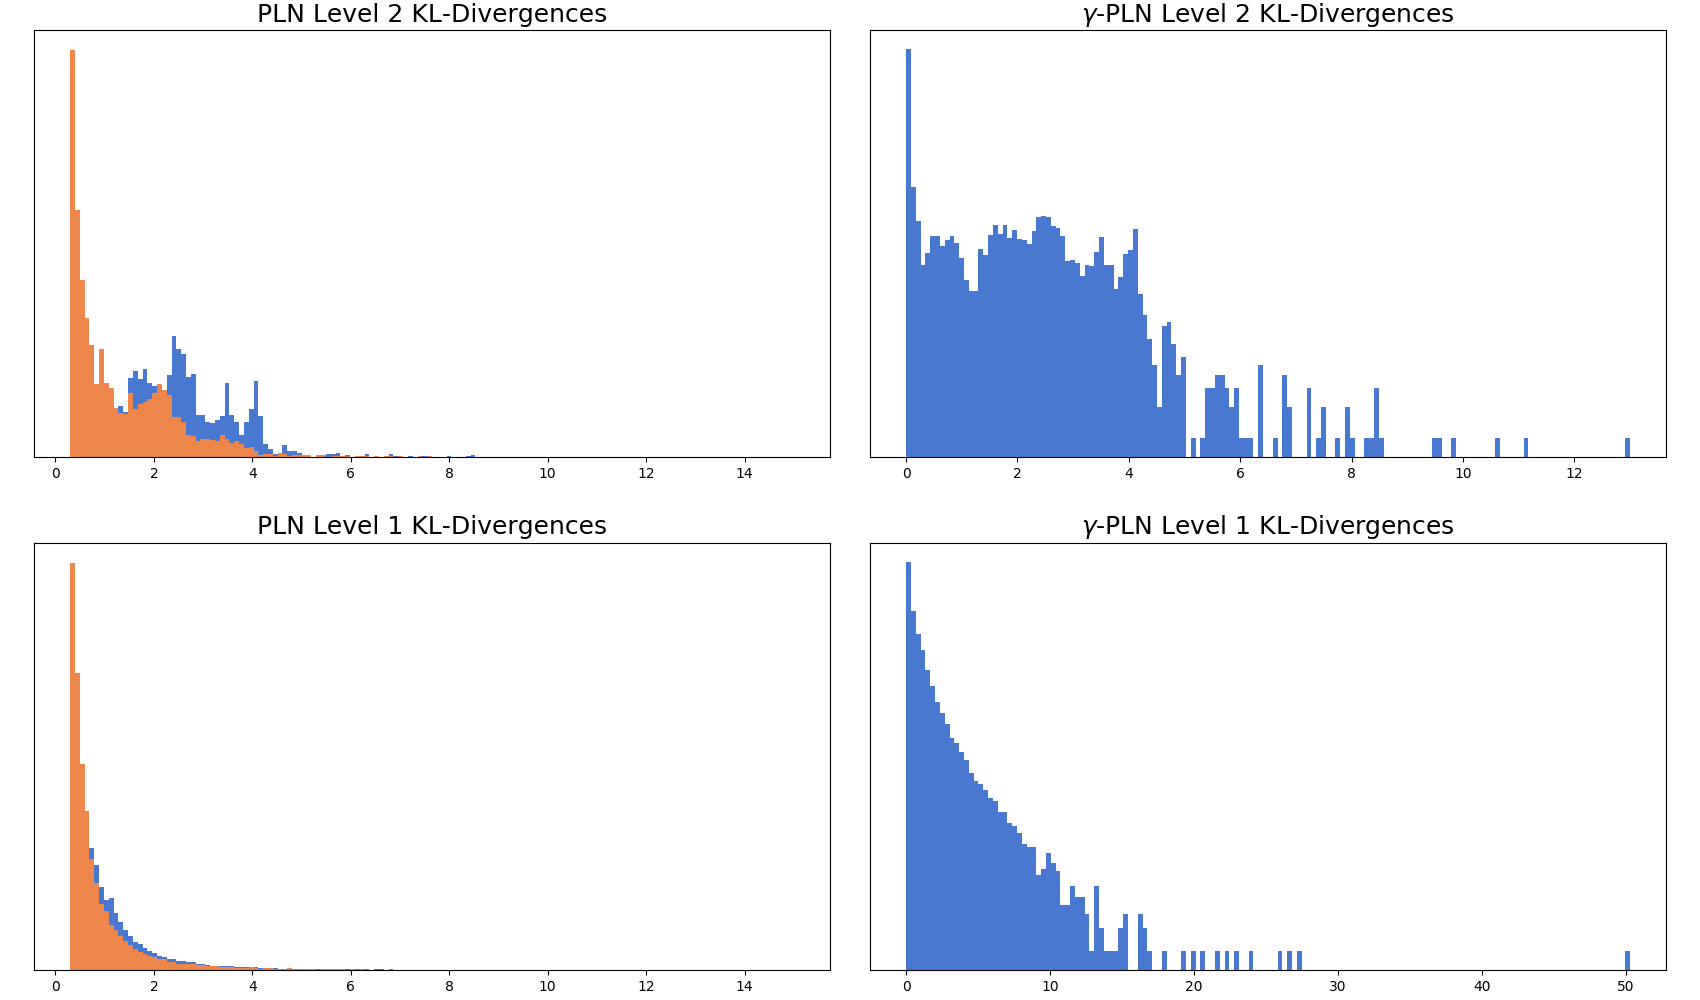
\includegraphics[width=\textwidth]{../img/plots/vae_latents/ladder_gamma_kl_comp}
  \caption{ladder on kodim21}
  \label{fig:ladder_gamma_kl_comp}
\end{figure}
\begin{figure}[H]
  \centering
  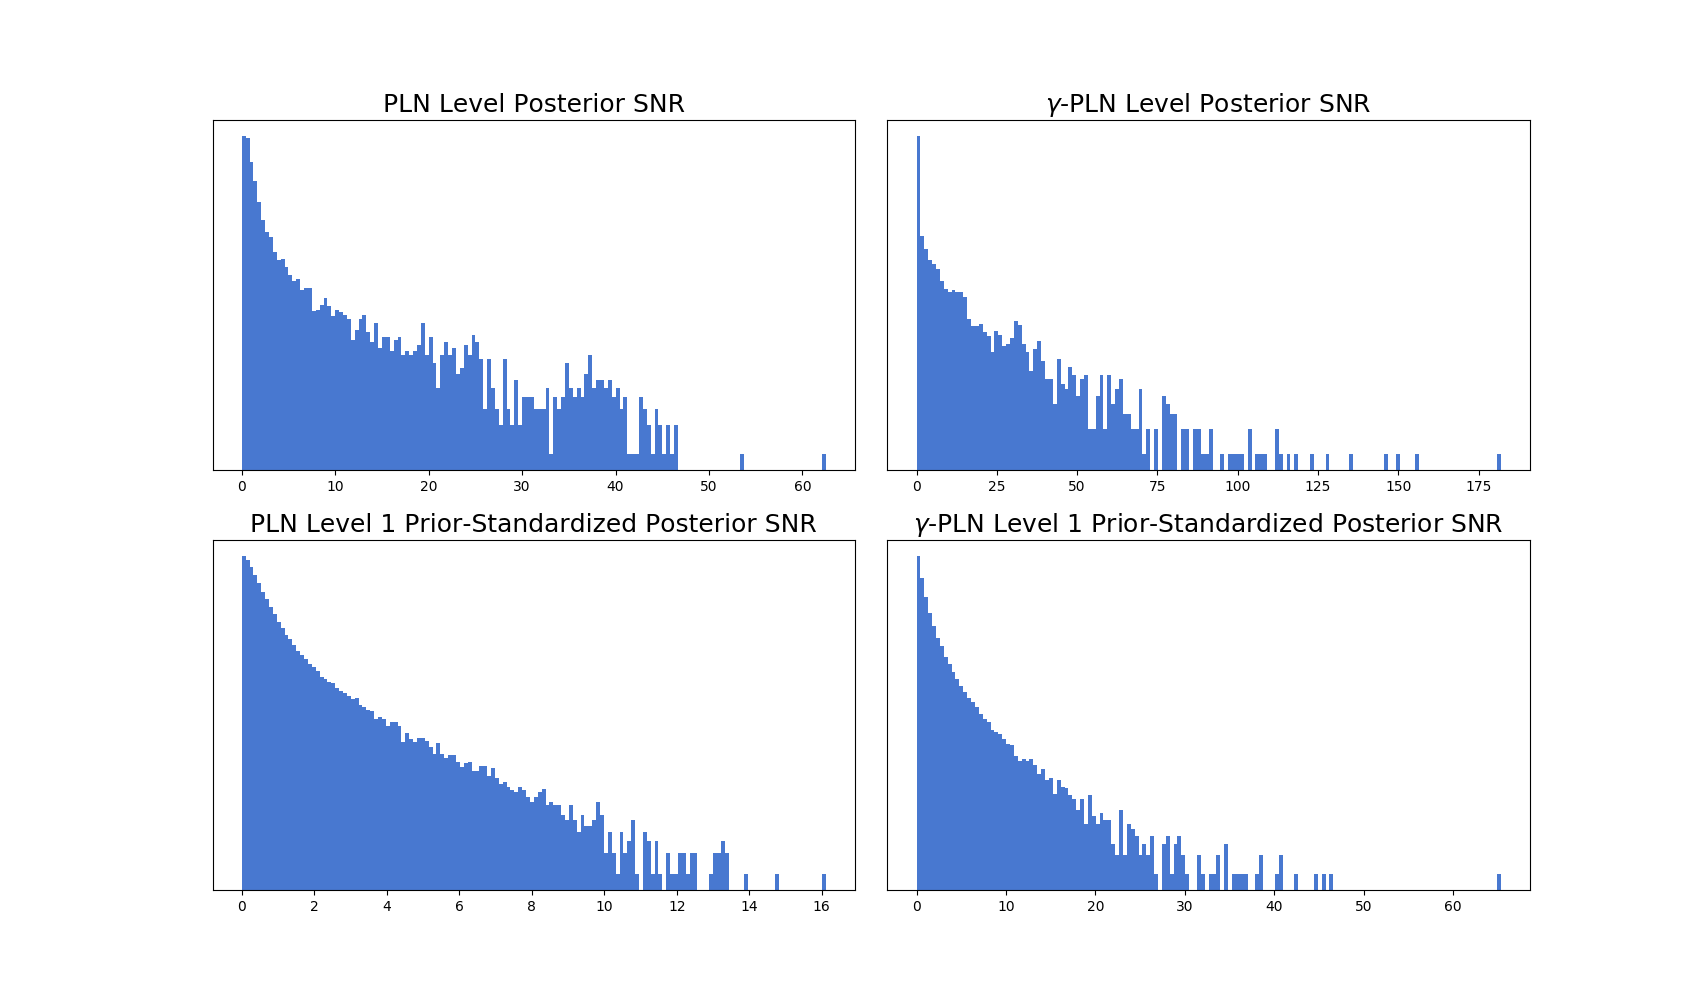
\includegraphics[width=\textwidth]{../img/plots/vae_latents/ladder_gamma_snr_comp}
  \caption{ladder on kodim21}
  \label{fig:ladder_gamma_snr_comp}
\end{figure}

\subsection{Compression Speed}
\par
Although not a focus of our project, we now briefly examine the the encoding and
decoding speed of our method. We have plotted the compression ratios of our
models against the time it took them to encode / decode them using IS-GS in
Figure \ref{fig:kodim01_coding_time}. As increasing the reconstruction quality
leads to higher KL divergences between the latent posteriors and priors, both the
importance sampler and the greedy sampler will need to split up a higher total
KL, and thus we expect the coding to become slower. This is precisely what we
observe, with a seemingly approximately linear growth, although we do not have
data to conclude this. We also see that encoding consistently takes around 3
times as long as decoding. It is clear that our method is not yet practical:
even the fastest case takes around a minute to encode and about 20 seconds to
decode, which very far away for real-time applications for now. The precise
values are reported in Table \ref{tab:kodim01_coding_time}.
\begin{figure}
  \centering
  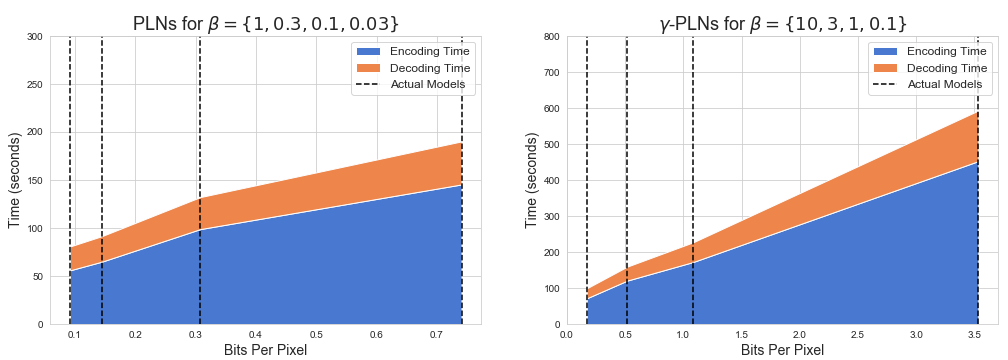
\includegraphics[width=\textwidth]{../img/plots/kodak_coding_time/kodim01_coding_time}
  \caption{Coding times of models plotted agains their rates. \textbf{Left:}
    Regular PLNs. \textbf{Right:} $\gamma$-PLNs. The striped lines indicate
    the concrete positions of our models in the rate line. While it seems
    that there is a
    linear relationship between rate and coding time, we do not have enough
    datapoints to conclude this.}
  \label{fig:kodim01_coding_time}
\end{figure}

\begin{table}[]
  \centering
  \begin{tabular}{|r||c|c|c|c||c|c|c|c|}
    \hline
    & \multicolumn{4}{c||}{\textbf{PLNs}} & \multicolumn{4}{c|}{\textbf{$\gamma$-PLNs}} \\
    \hline 
    $\beta$ & 1 & 0.3 & 0.1 & 0.03 & 10 & 3 & 1 & 0.1 \\ 
    \hline\hline
    Encoding Time (s) & 55.91 & 64.95 & 98.85 & 145.38 & 71.40 & 120.54 & 172.34 & 452.49 \\
    \hline
    Decoding Time (s) & 24.85 & 26.61 & 33.34 & 44.85 & 27.81 & 38.87 & 54.86 & 140.52 \\
    \hline
  \end{tabular}
  \caption{haha}
  \label{tab:kodim01_coding_time}
\end{table}




% EXPERIMENT TODO:
% comparison of different sized images' coding
% Balle hyperprior efficiency plot
% Sonderby latent KL plot
% latent variance plot

\section{Discussion}
\par
\section{Conclusion}
\par

\cite{townsend2019practical}
\printbibliography

\newpage

\section*{Appendix A: Sampling algorithms}
\subsection*{Rejection Sampling}
\par
The rejection sampling algorithm presented here is due to
\cite{harsha2007communication}.

\begin{algorithm}
  \caption{Rejection sampling presented in \cite{harsha2007communication}.}
  \label{alg:harsha_rej_sampling}
  \begin{algorithmic}[1]
    \Procedure{Rej-Sampler}{$P, Q, \langle x_i \sim Q \mid i \in \Nats \rangle$}
    \Comment $P$ is the prior
    \Statex
    \Comment $Q$ is the posterior
    \Statex
    \Comment $x_i$ are i.i.d. samples from $Q$
    \State $p_0(x) \gets 0 \quad \forall x \in \X$.
    \State $p_0^* \gets 0$.
    \For{$i \gets 1, \hdots \infty$}

    \State
    $\alpha_i(x) \gets \min{P(x) - p_{i - 1}(x), (1 - p_{i - 1}^*)Q(x)}\quad
    \forall x \in \X$

    \State $p_i(x) \gets p_{i - 1}(x) + \alpha_i(x)$
    
    \State $p_i^* \gets \sum_{x \in \X}p_i(x)$

    \State $\beta_i(x_i) \gets \frac{\alpha_i(x)}{(1 - p_i^*)Q(x)}$

    \State Draw $u \sim \Unif{0, 1}$

    \Statex

    \If{$u < \beta_i(x_i)$}

    \State\Return $i, x_i$

    \EndIf
    
    \EndFor
    \EndProcedure
  \end{algorithmic}
\end{algorithm}

\begin{algorithm}
  \caption{Importance sampling algorithm proposed by \cite{havasi2018minimal}}
  \label{alg:miracle_imp_samp}
  \begin{algorithmic}
    \Procedure{Importance-Sampler}{$P, Q, \langle x_i \sim Q \mid i \in \Nats \rangle$}
    \Comment $P$ is the prior
    \Statex
    \Comment $Q$ is the posterior
    \Statex
    \Comment $x_i$ are i.i.d. samples from $Q$

    \State $K \gets \exp\{\KL{Q}{P}\}$

    \State $\tilde{w}_i \gets \frac{Q(x_i)}{P(x_i)} \quad \forall i =
    1,\hdots K$

    \State Sample $j \sim p(\tilde{w})$

    \Return $j, x_j$
    \Statex
    \EndProcedure
  \end{algorithmic}
\end{algorithm}
\section*{Appendix B: Images}
\end{document}